\definecolor{datapolicy}{RGB}{68, 1, 84}
\definecolor{optimpolicy}{RGB}{49, 104, 142}

\definecolor{poptdraw}{RGB}{38, 130, 142}
\colorlet{poptd}{black!30!poptdraw}
\colorlet{poptds}{white!70!poptdraw}

\definecolor{naivetdraw}{RGB}{72, 40, 120}
\colorlet{naivetd}{black!30!naivetdraw}
\colorlet{naivetds}{white!70!naivetdraw}


\newcommand{\datapolicyglyph}[0]{\textls[10]{$\sqcdot\hspace{-.2em}\sqcdot\hspace{-.2em}\sqcdot$}}
\newcommand{\optimpolicyglyph}[0]{\raisebox{2pt}{\rule{8pt}{1.2pt}}}


A key problem in offline Reinforcement Learning (RL) is the mismatch between the dataset and the distribution over states and actions visited by the learned policy, called the \emph{distribution shift}. This is typically addressed by constraining the learned policy to be close to the data generating policy, at the cost of performance of the learned policy. We propose Projected Off-Policy TD (POP-TD), a new critic update rule that resamples TD updates to allow the learned policy to be distant from the data policy without catastrophic divergence. We show how various offline RL algorithms, notably Conservative Q-Learning (CQL), can be augmented to mitigate distribution shift. We evaluate our algorithm on some toy and small test cases, and set the stage for future work in this area.

\emph{Paper in preparation, by \citeauthor{manek2023poptd} (\citeyear{manek2023poptd})}

\clearpage


\section{Introduction}

Reinforcement Learning (RL) aims to learn policies that maximize rewards in Markov Decision Processes (MDPs) through interaction, generally using Temporal Difference (TD) methods. In contrast, offline RL focuses on learning optimal policies from a static dataset sampled from an unknown policy, possibly a policy designed for a different task. Thus, algorithms are expected to learn without the ability to interact with the environment.
This is useful in environments that are expensive to explore (such as running a Tokamak nuclear reactor \cite{degrave2022magnetic}), or high-dimensional environments with cheap access to expert or near-expert trajectories (such as video games). \citet{levine2020survey} present a comprehensive survey of the area.

Since in offline RL the data is gathered before training begins, there is a mismatch between the the state-distributions implied by the learned policy and the data.
When applying naive RL algorithms in this setting, they tend to bootstrap from regions with little or no data, causing runaway self-reinforcement.S
Offline RL algorithms like Conservative Q-Learning (CQL) \cite{kumar2020cql}, on the other hand, generally constrain the learned policy to remain within the support of the data. While this works well in practice, there still remains a large gap in performance between online and offline RL. One reason for this is an additional subtlety to distribution shift: because of the combination of off-policy RL and function approximation, it is possible for RL to diverge if the generating policy and the learned policy are sufficiently different.

\begin{figure}[t]
  \centering
  \begin{tikzpicture}
    \tikzset{
        table/.style={
                matrix of nodes,
                row sep=-\pgflinewidth,
                column sep=-\pgflinewidth,
                nodes={
                        rectangle,
                        draw=black,
                        align=center,
                        text width=2.5em,
                    },
                minimum height=2.5em,
                text depth=0.5ex,
                text height=2ex,
                nodes in empty cells,
            }
    }

    \matrix (m) [table,text width=6em]
    {
         &   &   & S \\
         & X &   & X \\
         &   &   &   \\
         &   & X & G \\
    };

    \draw [-to,color=datapolicy,line width=1.2pt,densely dotted]
    ([yshift=2pt,xshift=-4pt]m-1-4.center) -- ([yshift=2pt]m-1-1.center)
    ([yshift=2pt]m-1-1.center) -- (m-4-1.center)
    (m-4-1.center) -- (m-4-2.center)
    (m-4-2.center) -- ([yshift=-2pt]m-3-2.center)
    ([yshift=-2pt]m-3-2.center) -- ([yshift=-2pt,xshift=-3pt]m-3-4.center)
    ([yshift=-2pt,xshift=-3pt]m-3-4.center)[shorten >=4pt] -- ([xshift=-3pt]m-4-4.center);

    \draw [-to,color=optimpolicy,line width=1.2pt]
    ([yshift=-2pt,xshift=-4pt]m-1-4.center) -- ([yshift=-2pt]m-1-3.center)
    ([yshift=-2pt]m-1-3.center) -- ([yshift=2pt]m-3-3.center)
    ([yshift=2pt]m-3-3.center) -- ([yshift=2pt,xshift=3pt]m-3-4.center)
    ([yshift=2pt,xshift=3pt]m-3-4.center)[shorten >=4pt] -- ([xshift=3pt]m-4-4.center);

\end{tikzpicture}

  \caption{A simple grid environment illustrating distribution shift despite complete support. We wish to learn the optimal trajectory ({\color{optimpolicy} \optimpolicyglyph}) from a suboptimal data policy ({\color{datapolicy} \datapolicyglyph}) which is $\epsilon$-dithered to get sufficient coverage. When we apply Q-learning methods to this, training often diverges to arbitrarily poor values. This is a consequence of distribution shift. In this paper, we propose a technique to solve this divergence. }
  \label{fig:sopmap}
\end{figure}

We illustrate a simple case in Figure~\ref{fig:sopmap}, where a simple grid environment is designed to elicit the shortest trajectory from start (S) to goal (G). Agents can move one step in each cardinal direction, reaching the goal yields a unit reward, and the episode ends on reaching the goal or any marked cell (X). We generate a dataset by following a suboptimal data policy ({\color{datapolicy} \datapolicyglyph}) with sufficient dithering to guarantee that every state-action pair is represented. If we use a tabular Q-function, we can recover the optimal policy ({\color{optimpolicy} \optimpolicyglyph}) and obtain the true value function. When we use a linear Q-function, however, the error is much larger. We find that about half of random initializations lead to Q-functions that either diverge or converge to large error. This shows how even with full coverage of states and actions, distribution shift can be a significant source of error. We provide more details in Section~\ref{sec:expsimpleoffpolicy}.

\paragraph{Contributions}
In this chapter, we introduce POP-TD, a novel method of mitigating the error from off-policy learning. We show theoretically that this method bounds the off-policy approximation error for TD-based RL methods. We illustrate the resampling process on a well-known toy example, and then demonstrate its effectiveness on an example of offline RL under distribution shift.

\section{Related Work}

\paragraph{Off-Policy TD Learning} Instability from learning off-policy has also been studied in the classic RL literature.
First described by \citet{tsitsiklis1996analysis}, the use of TD learning, function approximation, and off-policy sampling may cause severe instability or divergence. This is known as the \emph{deadly triad} \citep[p.~264]{sutton2020reinforcement} and even if many variants of TD still converge, the quality of the solution at convergence may be arbitrarily poor \citep{kolter2011fixed}.


There are three existing lines of work in the literature that attempt to resolve this: regularization, Emphatic reweighing, and TD Distribution Optimization (TD-DO).
The first attempts to regularize TD, typically with $\mathcal L_2$-norm weight regularization. Alternative regularization schemes are $\mathcal L_1$ \citep{mahadevan2014proximal}, convex \citep{yu2017convergence}, and bounds propagation \citep{kumar2020discor}. There are well-documented failure modes related to regularization \cite{manek2022pitfalls}.
The second line started with Emphatic-TD, in which \citet{sutton2016emphatic} note that it is possible to reweigh samples obtained off-policy so they appear to be on-policy. Such methods learn the follow-on trace using Monte-Carlo methods (in the original), TD \citep{jiang2021learning,zhang2020provably} or techniques similar to TD \citep{hasselt2021expected}. The third method, TD-DO, works by solving a small optimization problem on each TD update to reweigh samples to satisfy the Non-Expansion Criterion, which we introduce in the next section.

\paragraph{Off-Policy and Offline Deep RL}

Nearly all modern TD-based deep RL methods perform off-policy learning in practice.
To improve data efficiency and learning stability, an experience replay buffer is often used. This buffer stores samples from an outdated version of the policy \citep{mnih2015humanlevel}.
Additionally, exploration policies, such as a epsilon greedy \citep[p.~100]{sutton2020reinforcement} or Soft Actor Critic (SAC)-style entropy regularization \citep{haarnoja2018soft} \footnote{While the original SAC algorithm is technically on-policy since it learns an entropy-regularized value function, the entropy-regularization is often dropped from the value-function estimate in practice to improve performance.}, are often used, which also results in off-policy learning.
In practice, the difference between the current policy and the samples in the buffer is limited by setting a limit to the buffer size and discarding old data; or by keeping the exploration policy relatively close to the learned policy. In practice, this is sufficient to prevent outright divergence, though the extent to which it decreases performance is not well-understood.

However, in the offline RL setting where training data is static, there is usually a much larger discrepancy between the state-action distribution of the data and the distribution induced by the learned policy.
This discrepancy presents a significant challenge for offline RL \citep{levine2020survey}.
While this distributional discrepancy is often presented as a single challenge for offline RL algorithms, there are two distinct aspects of this challenge that can be addressed independently: \textit{support mismatch} and \textit{proportional mismatch}.
When the support of the two distributions differ, learned value functions will have arbitrarily high errors in low-data regions.
Support mismatch is dealt with by either constraining the KL-divergence between the data and learned policies \citep{fujimoto2019off, kumar2019stabilizing, wu2019behavior}, by penalizing or pruning low-support (or high-uncertainty) actions \citep{kumar2020cql, yu2020mopo, kidambi2020morel}.

Even when the support of the data distribution matches that of the policy distribution, naive TD methods can produce unbounded errors in the value function \citep{tsitsiklis1996analysis}.
We call this challenge \textit{proportional mismatch}.

Importance sampling (IS) \citep{precup2000eligibility} is one of the most widely used techniques to address proportional mismatch.
The idea with IS is to compute the differences between the data and policy distributions for every state-action pair and re-weight the TD updates accordingly.
However, these methods suffer from variance that grows exponentially in the trajectory length.
Several methods have been proposed to mitigate this challenge and improve performance of IS in practice \citep{hallak2017consistent, gelada2019off, nachum2019dualdice, nachum2019algaedice, liu2018breaking}, but the learning is still far less stable than other offline deep RL methods.
In this work, we propose a new method to bound the value-function approximation errors caused by proportional mismatch without the need to explicitly compute (or approximate) IS weights.


%%%%%%%%%%%%%%%%%%%%%%%%%%%%%%%%%%%%%%%%%%%%%%%%%%%%%%%%%%%%

\section{Problem Setting and Notation }

Consider the $n$-state Markov chain $(\mathcal S, P, R, \gamma)$, with state space $\mathcal S$, transition function $P : \mathcal{S} \times \mathcal{S} \to \mathbb{R}_+$, reward function $R : \mathcal S \to \mathbb R$, and discount factor $\gamma \in [0, 1]$.
% $P \in \mathbb R^{n\times n}$ is the transition matrix, with $P_{ij}$ encoding the probability of moving from state $i$ to $j$.
Because the state-space is finite, it can be indexed as $\mathcal{S} = \{1, \ldots, n\}$.
This allows us to use matrix rather than operator notation.
The expected $\gamma$-discounted future reward of being in each state $V(s) \coloneqq \E \left[\left.\sum_{t=0}^\infty \gamma^t R(s_t) \right| s_0 = s \right]$ is called the value function.
The value function is consistent with Bellman's equation (in matrix form):
\begin{align}
  V = R + \gamma P V .
\end{align}
In the linear setting, we approximate the value function as $V(s) \approx w^\top \phi(s)$, where $\phi : \mathcal S \to \mathbb R^{k}$ is a fixed basis function and we estimate parameters $w \in \mathbb R^k$. In matrix notation, we write this as $V \approx \Phi w$.

In this work, we are interested in the offline learning setting, where the sampling distribution $\mu$ differs from the stationary distribution $\nu$.
In this setting, the TD solution is:
\begin{align}
  \Phi w & = \Pi_{\mu} (R + \gamma P \Phi w) ,
\end{align}
where $\Pi_\mu = \Phi(\Phi^\top D_{\mu} \Phi)^{-1}\Phi^\top D_{\mu}$ is the projection onto the column space of $\Phi$ weighted by the data distribution $\mu$ through the matrix $D_{\mu} = \diag(\mu)$. This projection may be arbitrarily far from the true solution, and so the error may be correspondingly large. The literature bounds the error as:
\begin{theorem}
  The error at the TD fixed point is $\|\Phi w - V \|_{D_\mu}$. Lemma 6 from \cite{tsitsiklis1996analysis} bounds this in terms of error projecting $V$ onto the column space of $\Phi$:
  \begin{align}
    \|\Phi w - V \|_{D_\mu} & \leq \frac{1}{1-\gamma} ~ \| \Pi_{\mu} V - V \|_{D_\mu}
  \end{align} \label{thm:boundTDError}
\end{theorem}

\subsection{Kolter's Non-Expansion Criterion (KNEC)}
Thus far we have left open the notion of a ``safe'' distribution to resample TD updates to. The on-policy distribution must be safe, but we need to establish a criteria for acceptable off-policy distributions. \citeauthor{tsitsiklis1996analysis} lay the groundwork for this by analyzing the training of on-policy TD as a dynamical system and showing that once TD reaches its fixed point, subsequent TD updates form a non-expansive mapping around that fixed point (\citeyear[lemma 4]{tsitsiklis1996analysis}), and therefore prove that on-policy TD does not diverge.

To do this, they begin with the fact that error bounds from on-policy TD follow the property that the $D-$norm of any vector $x \in \mathbb R^n$ is non-expansive through the transition matrix. That is: $\|Px\|_D \leq \|x\|_D$, where $D = \diag(\pi)$. \citet{kolter2011fixed} extend this analysis to the off-policy case, deriving a linear matrix inequality (LMI) under which the TD updates are guaranteed to be non-expansive around the fixed point. This is Kolter's Non-Expansion Criterion (\citeyear{kolter2011fixed}):
\begin{align}
  \|\Phi w - V\|_D                  & \leq \frac{1 + \gamma \kappa(D^{-\sfrac{1}{2}}D^{\sfrac{1}{2}})}{1 - \gamma} \|\Pi_D V - V\|_D
  \intertext{From this bound, he derives \emph{Kolter's non-expansion condition}:}
  \|\Pi_D P\Phi w\|_D               & \leq \|\Phi w\|_D \qquad (\forall w \in \mathbb R^n) \label{eqn:kolterthm2bound}
  \intertext{This holds if and only if the matrix $F_D$ is positive semi-definite}
  F_D                               & \equiv \begin{bmatrix}
                                               \Phi^\top D \Phi        & \Phi^\top D P \Phi \\
                                               \Phi^\top P^\top D \Phi & \Phi^\top D \Phi
                                             \end{bmatrix} \succcurlyeq 0
  \intertext{Equivalently, in terms of the expectation over states:}
  \E_{s\sim \mu, s'\sim p(\cdot|s)} & \left[\begin{bmatrix}
                                                \phi(s)\phi(s)^\top  & \phi(s)\phi(s')^\top \\
                                                \phi(s')\phi(s)^\top & \phi(s)\phi(s)^\top
                                              \end{bmatrix}\right] \succcurlyeq 0 . \label{eqn:knec}
\end{align}
This constraint describes a convex subset of $D$. As a $2k\times 2k$ matrix (where $k$ is the number of features), $F$ is prohibitively large to enumerate for any real RL problem, and so our algorithm is designed to make use of this without ever constructing it directly. Further, we notice that the construction of $F_D$ depends on $P$, the transition matrix of the underlying Markov process, which complicates how we construct it from samples.

For convenience, we write this as:
\begin{align}
   & \E_{s\sim q}  [F(s)] \succcurlyeq 0 \text{, where}                            \\
   & F(s) = \E_{s'\sim p(s'|s)}  \left[\begin{bmatrix}
                                           \phi(s)\phi(s)^\top  & \phi(s)\phi(s')^\top \\
                                           \phi(s')\phi(s)^\top & \phi(s)\phi(s)^\top
                                         \end{bmatrix}\right] . \label{eqn:fmatrix}
\end{align}
KNEC is an expectation over some state distribution $q$ and transition distribution $p(s,s') = p(s'|s) \mu(s)$. Because it is an LMI, the satisfying state distributions $q$ form a convex subset.

Directly constructing $F(s)$ or $F(s, s')$ is impossible on all but the simplest examples -- it would take $\mathcal O(k^2n)$ or $\mathcal O(k^2n^2)$ memory to hold all the necessary data. Instead we exploit the structure inherent in the problem to make use of $F(s)$ without creating it.


%%%%%%%%%%%%%%%%%%%%%%%%%%%%%%%%%%%%%%%%%%%%%%%%%%%%%%%%%%%%

\section{Projected Off-Policy TD (POP-TD) }

We propose an alternative approach to stabilizing off-policy training, based on Kolter's Non-Expansion Criterion \citep{kolter2011fixed}. POP-TD identifies a convex set of ``safe'' distributions that satisfy KNEC and reweighs TD updates to come from that set. In contrast to TD-DO, POP-TD uses solves a different optimization problem using a two-timescales update with fixed cost per iteration, allowing it to scale to real-world problems.

We begin by deriving the projected off-policy update for Markov Chains, without a separate policy function. We will extend this derivation to support actions and Markov Decision Processes (MDPs) in Section~\ref{sec:popq}. Our algorithm resamples TD updates so they come from some distribution $q$ for which KNEC holds. Given input data $(x_1, x_2, \ldots)$, this is the same as finding a set of weights $q_1, q_2, \ldots$ such that
\begin{align}
  \sum_i q_i & \cdot F(x_i) \succcurlyeq 0
\end{align}
% We also need to constrain our choice of distribution $q$ to ensure the quality of the solution.


\subsection{I- and M-projections} \label{sec:improj}
The Kullback-Leibler divergence is an \emph{asymmetric} measure, and so it is usually the case that $\min_q~\text{KL}(q||\mu) \neq \min_q~\text{KL}(\mu||q)$. The former (``from $\mu$ to $q$'') is an information (or I-)projection, which tends to under-estimate the support of $q$ potentially excluding possible sampling distributions to reweigh to. The latter (``from $q$ to $\mu$'') is a moment (or M-)projection, which tends to over-estimate the support of $q$ and avoid zero solutions. In our solution, we are proposing using an I-projection instead of the M-projection used by \citet{kolter2011fixed}.


\subsection{Optimizing the distribution}
\label{sec:distriboptim}

In the previous section we have characterized a convex subset of off-policy distributions under which TD learning is guaranteed not to diverge. If we can discover any such distribution for a particular TD problem, we can reweigh our TD updates (from any distribution) so they appear consistent with this reweighing distribution. This is related to the main insight in Emphatic-TD \citep{sutton2016emphatic}, with the key innovation that we can take any non-expansive distribution \emph{not just the on-policy distribution}.

We can now write down the optimization problem that we wish to solve:
\begin{align}
  \underset{q}{\text{minimize}}~\text{KL}(q||\mu) & \qquad \text{s.t. } ~ E_{s\sim q}[F(s)] \succcurlyeq 0
\end{align}
We are searching for $q$, the closest distribution to the sampling distribution $\mu$ such that $F$ is PSD under $q$. Note that we could in principle minimize any notion of ``closest'' to find some satisfying distribution -- for example \citet{kolter2011fixed} explores the effects of minimizing $\text{KL}(\mu||q)$.

We construct the dual of this problem:
\begin{align}
  \underset{Z\succcurlyeq 0}{\text{maximize}}~ \underset{q}{\text{minimize}}~\text{KL}(q||\mu) - \tr Z^\top \E_{s\sim q}[F(s)]
\end{align}
Using the Lagrange multiplier $Z\in\mathbb R^{2k\times 2k}$, we solve the inner optimization problem:
\begin{align}
  \underset{q}{\text{minimize}} - H(q) - \E_{s\sim q}[\log \mu(s) + \tr Z^\top F(s)]
\end{align}
Writing down Lagrangian and solving for the optima, we obtain:
\begin{align}
  q^*(s) & \propto \mu(s)\exp( \tr Z^\top F(s))
\end{align}
(Subject to the constraint that $q^*(s)$ is normalized so it must sum to 1 over all $s$.)

Plugging this back into our dual formulation, we obtain the optimization problem:
\begin{align}
  \underset{Z\succcurlyeq 0}{\text{maximize}}   & -\log \E_{s\sim\mu} [ \exp(\tr Z^\top F(s)) ]
  \intertext{Which we can simplify to}
  \underset{Z\succcurlyeq 0}{\text{minimize}} ~ & \E_{s\sim\mu} [ \exp(\tr Z^\top F(s)) ]
\end{align}

As discussed earlier, $F(s)$ cannot be directly constructed; instead, we assume that $Z$ holds a specific structure and optimize the problem.


\subsection{The structure of Z}

Our next goal is to transform this constrained optimization problem into an unconstrained problem over a low-rank version of $Z$, suitable for learning via SGD.

We assume (and later check!) that the solution for $Z$ is low-rank. Intuitively, this is because $\E_{s\sim\mu}[F(s)]$ is PSD when $\mu$ is close to $\pi$, and for most MDPs, sampling off-policy leads to only a small number of negative eigenvalues that need to be corrected by $Z$. \citet{kolter2011fixed} provides a technical explanation: by the KKT conditions, $Z$ will have rank complementary to $\E_{s\sim\mu}[F(s)]$, and the latter is expected to be full rank. It is worth noting that this ``almost-PSD'' assumption is common in the field.

We make the strong assumption that $Z$ has rank $m$, where $m << k$. We apply the Burer-Montiero approach \citep{burer2003nonlinear} to convert the constrained optimization problem over $Z$ into an unconstrained optimization over matrices $A\in \mathbb R^{k\times m}$ and $B\in \mathbb R^{k\times m}$:
\begin{align}
  Z^\star & = \begin{bmatrix} A \\ B \end{bmatrix} \begin{bmatrix} A \\ B\end{bmatrix}^T
\end{align}
This allows us to represent the rank-$m$ PSD matrix $Z^*$ in terms of the unconstrained matrices $A$ and $B$. Substituting this into the dual formulation, we get:
\begin{align}
  \underset{y}{\text{minimize}} & \;\; \mathbf{E}_{s\sim\mu} \left [ \exp\left (\tr  \begin{bmatrix} A \\ B \end{bmatrix} \begin{bmatrix} A \\ B \end{bmatrix}^T F(s) \right )  \right ]
\end{align}

We can leverage the structure of $F(s)$ to simplify the trace term:
\begin{align}
   & \tr Z^T F(s)
  \\ & = \tr \begin{bmatrix} A \\ B \end{bmatrix}^T \begin{bmatrix} A \\ B \end{bmatrix}^T F(s)
  \\ & = \tr \begin{bmatrix} A \\ B \end{bmatrix}^T F(s) \begin{bmatrix} A \\ B \end{bmatrix}
  \\ & = \tr \begin{bmatrix} A \\ B \end{bmatrix}^T  \mathbf{E}_{s' \sim p(s'|s)}  \left[ \begin{array}{cc} \phi(s)\phi(s)^T & \phi(s)\phi(s')^T \\ \phi(s')\phi(s)^T & \phi(s)\phi(s)^T \end{array} \right]
  \begin{bmatrix} A \\ B \end{bmatrix}
  \\  & = \tr \left[
    (A + B)^T \phi(s)\phi(s)^T (A+B)
    - 2B^T \mathbf{E}_{s' \sim p(s'|s)} \left [\phi(s)(\phi(s)- \phi(s'))^T \right ] A
    \right]
  \\  & = \| (A + B)^T \phi(s) \|^2 - \tr \left[
    2B^T \mathbf{E}_{s' \sim p(s'|s)} \left[ \phi(s)(\phi(s)- \phi(s'))^T \right] A
    \right]
\end{align}


This allows us to rewrite the optimization problem as:
\begin{align}
  \underset{y}{\text{minimize}} & \;\; \mathbf{E}_{s\sim\mu} \left [ \exp\left(
    \begin{array}{l}
      \| (A + B)^T \phi(s) \|^2
      \\ \qquad- \tr \left[
        2B^T \mathbf{E}_{s' \sim p(s'|s)} \left[ \phi(s)(\phi(s)- \phi(s'))^T \right] A
        \right]
    \end{array}
    \right) \right ]
\end{align}
where the small parameters $A$ and $B$ can be optimized with regular gradient-descent methods.


\subsection{Update rules}

We can't directly optimize our problem because that would require us to estimate the inner expectation term. Instead, we use a two-timescales approach by estimating two (dependent) quantities separately and improving them at potentially different rates. This (with a little tuning) can generally converge to a valid solution.

We choose to estimate the matrices $A, B \in \mathbb R^{k\times m}$ and separately the function $g_\theta : \mathcal S \in \mathbb R$ where
\begin{align}
  g_\theta(s) & \approx \tr Z^T F(s)
\end{align}
which can be approximated as a linear function (or a neural network) with parameters $\theta$. The size of the weights learned by POP-TD are therefore $\mathcal O(k)$, comparable to the size of vanilla Q-learning.

This corresponds to the auxiliary loss term for $A, B$:
\begin{align}
  \mathcal L_{A,B}(s, s')
   & = \exp(g_\theta(s)) \left [
    \| (A + B)^T \phi(s) \|^2 - \tr \left[
      2B^T \phi(s)(\phi(s)- \phi(s'))^T A
      \right]
    \right ]
  \intertext{and for $g$:}
  \mathcal L_{g}(s, s')
   & = \left( g_\theta(s) -
  \left [
      \| (A + B)^T \phi(s) \|^2 - \tr \left[
        2B^T \phi(s)(\phi(s)- \phi(s'))^T A
        \right]
      \right ]
  \right)^2
\end{align}

And finally, to complete this, we multiply each update of $w$ by $\exp(g(s))$ to resample it so it appears to come from the ``safe'' distribution, which completes the description of the algorithm!

\paragraph{Computing the loss} A naive implementation of the loss function will require intermediate matrices of size $[k\times k]$. We can improve speed by computing the loss in terms of $[m\times k]$ intermediates instead. For some $(s, s')$, this can be done as:
\begin{align}
  M_A & = A^T \phi(s) \in \mathbb R^{m\times k} \nonumber
  \\  M_A' & = A^T \phi(s') \in \mathbb R^{m\times k} \nonumber
  \\  M_B & = B^T \phi(s) \in \mathbb R^{m\times k} \nonumber
  \\  \mathcal L_{A,B}(s, s') & \equiv \exp(g_\theta(s)) \left [
    \| M_A + M_B \|^2
    - 2 (M_A - M_A') \cdot M_B
    \right ]
  \\    \mathcal L_{g}(s, s') & \equiv \left( g_\theta(s) -\left [
      \| M_A + M_B \|^2
      - 2 (M_A - M_A') \cdot M_B
      \right ]
  \right)^2
\end{align}
where $\cdot$ is the dot product. This sequence of operations should be $\mathcal O(m^2 k)$, which is much quicker than the naive $\mathcal O(m k^2)$.

\subsection{POP-Q-Learning}\label{sec:popq}\label{sec:pop-q-derivation}

Thus far, we have focused on Markov Reward Processes.
For RL problems, we need to extend this approach to Markov Decision Processes (MDPs).
% We now extend this from simple Markov chains to MDPs by incorporating actions into it.
An MDP is a tuple, $(\mathcal{S}, \mathcal{A}, P, R, \gamma)$, with state space $\mathcal S$, transition function $P : \mathcal{S} \times \mathcal{A} \times \mathcal{S} \to \mathbb{R}_+$, reward function $R : \mathcal S \times \mathcal{A} \to \mathbb R$, and discount factor $\gamma \in [0, 1]$.
The goal in this setting is to find a probabilistic policy $\pi : \mathcal{S} \times \mathcal{A} \to \mathbb{R}_+$ that maximizes the future discounted reward:
\begin{equation}
  \pi^\star = \argmax_\pi \E_\pi \left [ \sum_{t=0}^\infty \gamma^t R(s_t, a_t) \right ]
\end{equation}
Many RL methods use variations of Q-learning \cite{watkins1992q,mnih2015humanlevel,haarnoja2018soft,kumar2020cql}, which involves learning a state-action value function, or $Q$-function:
\begin{equation}
  Q^\pi(s, a) = \E_\pi \left[\left.\sum_{t=0}^\infty \gamma^t R(s_t, a_t) \right| s_0 = s, a_0 = a \right]
\end{equation}

By considering a fixed policy $\pi$, a combined state-space $\mathcal{X} = \mathcal{S} \times \mathcal{A}$, and a policy-conditioned transition function $\tilde{P}^\pi((s, a), (s', a')) = P(s, a, s') \pi(s', a')$, any MDP reduces to a Markov Chain.
Thus, as long as the NEC is satisfied in this modified state-space, we can bound the approximation error of the Q-function.
See \cref{sec:pop-q-derivation} for a detailed derivation.

Finally, for our method to applied to modern deep RL problems, we must extend our approach to non-linear Q-functions.
To do so, we approximate the Q-function with a neural network, $Q_{\theta^Q}$ parameterized by $\theta^Q$ and consider a stochastic parameterized policy $\pi_{\theta^\pi}$.
To update $Q_{\theta^Q}$, we used a squared Bellman loss, $\mathcal{L}_Q(\theta^Q) = (Q_{\theta^Q}(s, a) - r - \gamma Q_{\theta^Q}(s', \pi_{\theta^\pi}(s')))^2$, which we reweigh with $e^{g(s)}$ as before.
For our offline RL experiments, we also add CQL regularization \citep{kumar2020cql} to our Q-learning updates to prevent over-optimism on low-support regions of the state-action space.
To update our linear dual variables $y$, we use the penultimate layer of $Q_{\theta^Q}$ as our feature vector.
Finally, we use a SAC-style entropy regularized loss to update our policy network, $\pi_{\theta^\pi}$.
\Cref{alg:example} provides an overview of our method.


\begin{algorithm}[tb]
  \caption{Deep POP-Q-Learning}
  \label{alg:example}
  \begin{algorithmic}
    \STATE  Initialize Q-function, $Q_{\theta^Q}$, g-function, $g_{\theta^g}$, dual variable vector $y$, and some policy $\pi_{\theta^\pi}$.
    \FOR{step $t$ in ${1, \ldots, N}$}
    \STATE Sample mini-batch $(s, a, r, s') \sim \mu$.
    \STATE Sample $\tilde{a} \sim \pi_{\theta^\pi}(s), \tilde{a}' \sim \pi_{\theta^\pi}(s')$.
    \STATE \# Compute features from penultimate layer of Q-network:
    \STATE $\phi \gets Q_{\theta^Q}(s, a), \phi' \gets Q_{\theta^Q}(s', \tilde{a}')$.
    \STATE \# Update g-function and dual variable vectors:
    \STATE $\theta^g_t \gets \theta^g_{t-1} - \eta_g \nabla_{\theta^g} \mathcal{L}_g(s, s')$
    \STATE $A_t \gets A_{t-1} - \eta_A \nabla_{A} \mathcal{L}_{A}(s, s')$
    \STATE $B_t \gets B_{t-1} - \eta_B \nabla_{B} \mathcal{L}_{B}(s, s')$
    \STATE \# Update Q-function using re-weighted Q-loss update:
    \STATE $\theta^Q_t \gets \theta^Q_{t-1} - \eta_Q \exp (g_{\theta^g}(s, a)) \nabla_{\theta^Q} \mathcal{L}_Q(\theta^Q)$
    \STATE \# Update policy with SAC-style loss:
    \STATE $\theta^\pi_t \gets \theta^\pi_{t-1} - \eta_\pi \nabla_{\theta_\pi} [Q_{\theta^Q}(s, \tilde{a}) - \log \pi_{\theta^\pi}(\tilde{a} | s)]$
    \ENDFOR
  \end{algorithmic}
\end{algorithm}

\section{Experiments and Discussion}

We first apply POP-TD to a well-understood example so that we can directly illustrate the how it resamples TD updates to a ``safe'' distribution. We use the simple three-state task from \cref{fig:threestate}, including the specified transition function, value function, and basis. Since this is a policy evaluation task, there is no policy to be separately learned.

For illustration purposes, we select the family of distributions $\pi = (\sfrac h 2, \sfrac h 2, 1- h)$ parameterized by $h \in [0, 1]$.
This characterizes the possible distributions of data that we will present to POP-TD and naive TD in this experiment. The on-policy distribution corresponds to $h_o\approx 0.51$, and divides the family of distributions into a left subset ($h \leq h_o$) where KNEC holds and a right subset ($h_o > 0.5$) where KNEC does not. This is immediately apparent in \cref{fig:threestate}, where we plot the error at convergence from running naive- and POP-TD above, and the effective distribution of TD updates after reweighing below.
In the left subset, where KNEC holds, POP-TD does not resample TD updates at all. Therefore, the error of POP-TD tracks naive TD (top), and the effective distribution of TD updates in POP-TD and naive TD are the same as the data distribution (bottom).

In the right subset, we observe that naive TD converges to poor solutions with large error while POP-TD is able to learn with low error.
Directly computing the effective distribution, we see that naive TD adheres to the data distribution but POP-TD resamples the TD updates.
Looking at the behavior of POP-TD in the right subset, we see that POP-TD resamples updates to the on-policy distribution $p_o$ in $p\in[p_o,0.9]$, corresponding to the horizontal segment. This allows the learned Q-function to have very low error in that domain. As the data distribution becomes more extreme ($p\in [0.9, 1)$), POP-TD is not quite able to learn the resampling ratio, and so the effective distribution shifts away from $p_o$. This leads to a corresponding slight increase in error at extreme ratios. From this we observe that POP-TD requires full support of the sampling distribution, similar to many offline RL algorithms \cite{kumar2020cql,shi2022pessimistic}.

This simple experiment cleanly illustrates how POP-TD resamples TD updates to come from a ``safe'' distribution, and how that can greatly reduce the error in a policy evaluation task.

\label{sec:threestateexp}
\begin{figure}[t]
  \centering
  \begin{tikzpicture}
    \begin{groupplot}[
        group style={
                % set how the plots should be organized
                group size=1 by 2,
                % only show ticklabels and axis labels on the bottom
                x descriptions at=edge bottom,
                % set the `vertical sep' to zero
                vertical sep=0pt,
            },
        width=1.\columnwidth,
        height=.6\columnwidth,
        xmin=0, xmax=1,
        xlabel={Distrib. param. $h$, where $\pi = [\sfrac h 2, \sfrac h 2, 1-h]$},
        ]

        \nextgroupplot[
            ylabel={$\log_{10}$ Error},
            ymode=log,
            ymin=0.00001, ymax=1000,
            yticklabels={-5,-1,3}
        ]

        \addplot [color=poptd] table [x index=0,y index=1] {poptd/threestate/export_threestate.dat};
        \node at (axis cs:.75,0.0001) [anchor=south west,color=poptd] {POP-TD};

        \addplot [color=naivetd,dashed] table [x index=0,y index=2] {poptd/threestate/export_threestate.dat};
        \node at (axis cs:.75,1.) [anchor=north west,color=naivetd] {Naive TD};
        % \addlegendentry{Naive TD}

        \node at (axis cs:.514,1000) [anchor=north east] {$F(s)\succcurlyeq 0$};
        \node at (axis cs:.514,1000) [anchor=north west] {$F(s)\not\succcurlyeq 0$};
        \draw[dotted,thick] (axis cs:0.514,0.0000001) -- (axis cs:0.514,1000000);

        \nextgroupplot[
            ylabel={effective distrib. $p$},
            ymin=0., ymax=1.,
            yticklabels={,0,.2,.4,.6,.8,}
        ]

        \addplot [color=poptd] table [x index=0,y index=3] {poptd/threestate/export_threestate.dat};
        \node at (axis cs:.75,.5) [anchor=north east,color=poptd] {POP-TD};

        \addplot [color=naivetd, domain=0:1,dashed] {x} ;
        \node at (axis cs:.75,.75) [anchor=south east,color=naivetd] {Naive TD};

        \draw[dotted,thick] (axis cs:0.514,0.) -- (axis cs:0.514,1);

    \end{groupplot}

\end{tikzpicture}

  \caption{The error in the learned value function by naive- and POP-TD, plotted against a varying sampling distribution. In the left half of the plot, KNEC holds, and so POP-TD tracks the error of naive TD closely. In the right half of the plot naive TD diverges, while POP-TD resamples the data to a ``safe'' distribution and does not diverge. }
  \label{fig:threestate}
\end{figure}


\subsection{POP-Q on GridWorld}

\label{sec:expsimpleoffpolicy}
\begin{figure}[t]
  \centering
  %% Creator: Matplotlib, PGF backend
%%
%% To include the figure in your LaTeX document, write
%%   \input{<filename>.pgf}
%%
%% Make sure the required packages are loaded in your preamble
%%   \usepackage{pgf}
%%
%% Also ensure that all the required font packages are loaded; for instance,
%% the lmodern package is sometimes necessary when using math font.
%%   \usepackage{lmodern}
%%
%% Figures using additional raster images can only be included by \input if
%% they are in the same directory as the main LaTeX file. For loading figures
%% from other directories you can use the `import` package
%%   \usepackage{import}
%%
%% and then include the figures with
%%   \import{<path to file>}{<filename>.pgf}
%%
%% Matplotlib used the following preamble
%%   \usepackage{fontspec}
%%   \setmainfont{DejaVuSerif.ttf}[Path=\detokenize{/home/gauravmm/.pyenv/versions/3.9.7/envs/tddo/lib/python3.9/site-packages/matplotlib/mpl-data/fonts/ttf/}]
%%   \setsansfont{DejaVuSans.ttf}[Path=\detokenize{/home/gauravmm/.pyenv/versions/3.9.7/envs/tddo/lib/python3.9/site-packages/matplotlib/mpl-data/fonts/ttf/}]
%%   \setmonofont{DejaVuSansMono.ttf}[Path=\detokenize{/home/gauravmm/.pyenv/versions/3.9.7/envs/tddo/lib/python3.9/site-packages/matplotlib/mpl-data/fonts/ttf/}]
%%
\begingroup%
\makeatletter%
\begin{pgfpicture}%
\pgfpathrectangle{\pgfpointorigin}{\pgfqpoint{6.000000in}{4.000000in}}%
\pgfusepath{use as bounding box, clip}%
\begin{pgfscope}%
\pgfsetbuttcap%
\pgfsetmiterjoin%
\pgfsetlinewidth{0.000000pt}%
\definecolor{currentstroke}{rgb}{1.000000,1.000000,1.000000}%
\pgfsetstrokecolor{currentstroke}%
\pgfsetstrokeopacity{0.000000}%
\pgfsetdash{}{0pt}%
\pgfpathmoveto{\pgfqpoint{0.000000in}{0.000000in}}%
\pgfpathlineto{\pgfqpoint{6.000000in}{0.000000in}}%
\pgfpathlineto{\pgfqpoint{6.000000in}{4.000000in}}%
\pgfpathlineto{\pgfqpoint{0.000000in}{4.000000in}}%
\pgfpathlineto{\pgfqpoint{0.000000in}{0.000000in}}%
\pgfpathclose%
\pgfusepath{}%
\end{pgfscope}%
\begin{pgfscope}%
\pgfsetbuttcap%
\pgfsetmiterjoin%
\definecolor{currentfill}{rgb}{1.000000,1.000000,1.000000}%
\pgfsetfillcolor{currentfill}%
\pgfsetlinewidth{0.000000pt}%
\definecolor{currentstroke}{rgb}{0.000000,0.000000,0.000000}%
\pgfsetstrokecolor{currentstroke}%
\pgfsetstrokeopacity{0.000000}%
\pgfsetdash{}{0pt}%
\pgfpathmoveto{\pgfqpoint{0.750000in}{0.500000in}}%
\pgfpathlineto{\pgfqpoint{5.400000in}{0.500000in}}%
\pgfpathlineto{\pgfqpoint{5.400000in}{3.520000in}}%
\pgfpathlineto{\pgfqpoint{0.750000in}{3.520000in}}%
\pgfpathlineto{\pgfqpoint{0.750000in}{0.500000in}}%
\pgfpathclose%
\pgfusepath{fill}%
\end{pgfscope}%
\begin{pgfscope}%
\pgfpathrectangle{\pgfqpoint{0.750000in}{0.500000in}}{\pgfqpoint{4.650000in}{3.020000in}}%
\pgfusepath{clip}%
\pgfsetbuttcap%
\pgfsetmiterjoin%
\definecolor{currentfill}{rgb}{0.121569,0.466667,0.705882}%
\pgfsetfillcolor{currentfill}%
\pgfsetlinewidth{0.000000pt}%
\definecolor{currentstroke}{rgb}{0.000000,0.000000,0.000000}%
\pgfsetstrokecolor{currentstroke}%
\pgfsetstrokeopacity{0.000000}%
\pgfsetdash{}{0pt}%
\pgfpathmoveto{\pgfqpoint{0.961364in}{0.500000in}}%
\pgfpathlineto{\pgfqpoint{1.313636in}{0.500000in}}%
\pgfpathlineto{\pgfqpoint{1.313636in}{0.902667in}}%
\pgfpathlineto{\pgfqpoint{0.961364in}{0.902667in}}%
\pgfpathlineto{\pgfqpoint{0.961364in}{0.500000in}}%
\pgfpathclose%
\pgfusepath{fill}%
\end{pgfscope}%
\begin{pgfscope}%
\pgfpathrectangle{\pgfqpoint{0.750000in}{0.500000in}}{\pgfqpoint{4.650000in}{3.020000in}}%
\pgfusepath{clip}%
\pgfsetbuttcap%
\pgfsetmiterjoin%
\definecolor{currentfill}{rgb}{0.121569,0.466667,0.705882}%
\pgfsetfillcolor{currentfill}%
\pgfsetlinewidth{0.000000pt}%
\definecolor{currentstroke}{rgb}{0.000000,0.000000,0.000000}%
\pgfsetstrokecolor{currentstroke}%
\pgfsetstrokeopacity{0.000000}%
\pgfsetdash{}{0pt}%
\pgfpathmoveto{\pgfqpoint{1.313636in}{0.500000in}}%
\pgfpathlineto{\pgfqpoint{1.665909in}{0.500000in}}%
\pgfpathlineto{\pgfqpoint{1.665909in}{0.902667in}}%
\pgfpathlineto{\pgfqpoint{1.313636in}{0.902667in}}%
\pgfpathlineto{\pgfqpoint{1.313636in}{0.500000in}}%
\pgfpathclose%
\pgfusepath{fill}%
\end{pgfscope}%
\begin{pgfscope}%
\pgfpathrectangle{\pgfqpoint{0.750000in}{0.500000in}}{\pgfqpoint{4.650000in}{3.020000in}}%
\pgfusepath{clip}%
\pgfsetbuttcap%
\pgfsetmiterjoin%
\definecolor{currentfill}{rgb}{0.121569,0.466667,0.705882}%
\pgfsetfillcolor{currentfill}%
\pgfsetlinewidth{0.000000pt}%
\definecolor{currentstroke}{rgb}{0.000000,0.000000,0.000000}%
\pgfsetstrokecolor{currentstroke}%
\pgfsetstrokeopacity{0.000000}%
\pgfsetdash{}{0pt}%
\pgfpathmoveto{\pgfqpoint{1.665909in}{0.500000in}}%
\pgfpathlineto{\pgfqpoint{2.018182in}{0.500000in}}%
\pgfpathlineto{\pgfqpoint{2.018182in}{0.500000in}}%
\pgfpathlineto{\pgfqpoint{1.665909in}{0.500000in}}%
\pgfpathlineto{\pgfqpoint{1.665909in}{0.500000in}}%
\pgfpathclose%
\pgfusepath{fill}%
\end{pgfscope}%
\begin{pgfscope}%
\pgfpathrectangle{\pgfqpoint{0.750000in}{0.500000in}}{\pgfqpoint{4.650000in}{3.020000in}}%
\pgfusepath{clip}%
\pgfsetbuttcap%
\pgfsetmiterjoin%
\definecolor{currentfill}{rgb}{0.121569,0.466667,0.705882}%
\pgfsetfillcolor{currentfill}%
\pgfsetlinewidth{0.000000pt}%
\definecolor{currentstroke}{rgb}{0.000000,0.000000,0.000000}%
\pgfsetstrokecolor{currentstroke}%
\pgfsetstrokeopacity{0.000000}%
\pgfsetdash{}{0pt}%
\pgfpathmoveto{\pgfqpoint{2.018182in}{0.500000in}}%
\pgfpathlineto{\pgfqpoint{2.370454in}{0.500000in}}%
\pgfpathlineto{\pgfqpoint{2.370454in}{0.701333in}}%
\pgfpathlineto{\pgfqpoint{2.018182in}{0.701333in}}%
\pgfpathlineto{\pgfqpoint{2.018182in}{0.500000in}}%
\pgfpathclose%
\pgfusepath{fill}%
\end{pgfscope}%
\begin{pgfscope}%
\pgfpathrectangle{\pgfqpoint{0.750000in}{0.500000in}}{\pgfqpoint{4.650000in}{3.020000in}}%
\pgfusepath{clip}%
\pgfsetbuttcap%
\pgfsetmiterjoin%
\definecolor{currentfill}{rgb}{0.121569,0.466667,0.705882}%
\pgfsetfillcolor{currentfill}%
\pgfsetlinewidth{0.000000pt}%
\definecolor{currentstroke}{rgb}{0.000000,0.000000,0.000000}%
\pgfsetstrokecolor{currentstroke}%
\pgfsetstrokeopacity{0.000000}%
\pgfsetdash{}{0pt}%
\pgfpathmoveto{\pgfqpoint{2.370454in}{0.500000in}}%
\pgfpathlineto{\pgfqpoint{2.722727in}{0.500000in}}%
\pgfpathlineto{\pgfqpoint{2.722727in}{0.701333in}}%
\pgfpathlineto{\pgfqpoint{2.370454in}{0.701333in}}%
\pgfpathlineto{\pgfqpoint{2.370454in}{0.500000in}}%
\pgfpathclose%
\pgfusepath{fill}%
\end{pgfscope}%
\begin{pgfscope}%
\pgfpathrectangle{\pgfqpoint{0.750000in}{0.500000in}}{\pgfqpoint{4.650000in}{3.020000in}}%
\pgfusepath{clip}%
\pgfsetbuttcap%
\pgfsetmiterjoin%
\definecolor{currentfill}{rgb}{0.121569,0.466667,0.705882}%
\pgfsetfillcolor{currentfill}%
\pgfsetlinewidth{0.000000pt}%
\definecolor{currentstroke}{rgb}{0.000000,0.000000,0.000000}%
\pgfsetstrokecolor{currentstroke}%
\pgfsetstrokeopacity{0.000000}%
\pgfsetdash{}{0pt}%
\pgfpathmoveto{\pgfqpoint{2.722727in}{0.500000in}}%
\pgfpathlineto{\pgfqpoint{3.075000in}{0.500000in}}%
\pgfpathlineto{\pgfqpoint{3.075000in}{0.902667in}}%
\pgfpathlineto{\pgfqpoint{2.722727in}{0.902667in}}%
\pgfpathlineto{\pgfqpoint{2.722727in}{0.500000in}}%
\pgfpathclose%
\pgfusepath{fill}%
\end{pgfscope}%
\begin{pgfscope}%
\pgfpathrectangle{\pgfqpoint{0.750000in}{0.500000in}}{\pgfqpoint{4.650000in}{3.020000in}}%
\pgfusepath{clip}%
\pgfsetbuttcap%
\pgfsetmiterjoin%
\definecolor{currentfill}{rgb}{0.121569,0.466667,0.705882}%
\pgfsetfillcolor{currentfill}%
\pgfsetlinewidth{0.000000pt}%
\definecolor{currentstroke}{rgb}{0.000000,0.000000,0.000000}%
\pgfsetstrokecolor{currentstroke}%
\pgfsetstrokeopacity{0.000000}%
\pgfsetdash{}{0pt}%
\pgfpathmoveto{\pgfqpoint{3.075000in}{0.500000in}}%
\pgfpathlineto{\pgfqpoint{3.427273in}{0.500000in}}%
\pgfpathlineto{\pgfqpoint{3.427273in}{0.701333in}}%
\pgfpathlineto{\pgfqpoint{3.075000in}{0.701333in}}%
\pgfpathlineto{\pgfqpoint{3.075000in}{0.500000in}}%
\pgfpathclose%
\pgfusepath{fill}%
\end{pgfscope}%
\begin{pgfscope}%
\pgfpathrectangle{\pgfqpoint{0.750000in}{0.500000in}}{\pgfqpoint{4.650000in}{3.020000in}}%
\pgfusepath{clip}%
\pgfsetbuttcap%
\pgfsetmiterjoin%
\definecolor{currentfill}{rgb}{0.121569,0.466667,0.705882}%
\pgfsetfillcolor{currentfill}%
\pgfsetlinewidth{0.000000pt}%
\definecolor{currentstroke}{rgb}{0.000000,0.000000,0.000000}%
\pgfsetstrokecolor{currentstroke}%
\pgfsetstrokeopacity{0.000000}%
\pgfsetdash{}{0pt}%
\pgfpathmoveto{\pgfqpoint{3.427272in}{0.500000in}}%
\pgfpathlineto{\pgfqpoint{3.779545in}{0.500000in}}%
\pgfpathlineto{\pgfqpoint{3.779545in}{1.506667in}}%
\pgfpathlineto{\pgfqpoint{3.427272in}{1.506667in}}%
\pgfpathlineto{\pgfqpoint{3.427272in}{0.500000in}}%
\pgfpathclose%
\pgfusepath{fill}%
\end{pgfscope}%
\begin{pgfscope}%
\pgfpathrectangle{\pgfqpoint{0.750000in}{0.500000in}}{\pgfqpoint{4.650000in}{3.020000in}}%
\pgfusepath{clip}%
\pgfsetbuttcap%
\pgfsetmiterjoin%
\definecolor{currentfill}{rgb}{0.121569,0.466667,0.705882}%
\pgfsetfillcolor{currentfill}%
\pgfsetlinewidth{0.000000pt}%
\definecolor{currentstroke}{rgb}{0.000000,0.000000,0.000000}%
\pgfsetstrokecolor{currentstroke}%
\pgfsetstrokeopacity{0.000000}%
\pgfsetdash{}{0pt}%
\pgfpathmoveto{\pgfqpoint{3.779546in}{0.500000in}}%
\pgfpathlineto{\pgfqpoint{4.131818in}{0.500000in}}%
\pgfpathlineto{\pgfqpoint{4.131818in}{2.312000in}}%
\pgfpathlineto{\pgfqpoint{3.779546in}{2.312000in}}%
\pgfpathlineto{\pgfqpoint{3.779546in}{0.500000in}}%
\pgfpathclose%
\pgfusepath{fill}%
\end{pgfscope}%
\begin{pgfscope}%
\pgfpathrectangle{\pgfqpoint{0.750000in}{0.500000in}}{\pgfqpoint{4.650000in}{3.020000in}}%
\pgfusepath{clip}%
\pgfsetbuttcap%
\pgfsetmiterjoin%
\definecolor{currentfill}{rgb}{0.121569,0.466667,0.705882}%
\pgfsetfillcolor{currentfill}%
\pgfsetlinewidth{0.000000pt}%
\definecolor{currentstroke}{rgb}{0.000000,0.000000,0.000000}%
\pgfsetstrokecolor{currentstroke}%
\pgfsetstrokeopacity{0.000000}%
\pgfsetdash{}{0pt}%
\pgfpathmoveto{\pgfqpoint{4.131818in}{0.500000in}}%
\pgfpathlineto{\pgfqpoint{4.484090in}{0.500000in}}%
\pgfpathlineto{\pgfqpoint{4.484090in}{0.500000in}}%
\pgfpathlineto{\pgfqpoint{4.131818in}{0.500000in}}%
\pgfpathlineto{\pgfqpoint{4.131818in}{0.500000in}}%
\pgfpathclose%
\pgfusepath{fill}%
\end{pgfscope}%
\begin{pgfscope}%
\pgfpathrectangle{\pgfqpoint{0.750000in}{0.500000in}}{\pgfqpoint{4.650000in}{3.020000in}}%
\pgfusepath{clip}%
\pgfsetbuttcap%
\pgfsetmiterjoin%
\definecolor{currentfill}{rgb}{0.121569,0.466667,0.705882}%
\pgfsetfillcolor{currentfill}%
\pgfsetlinewidth{0.000000pt}%
\definecolor{currentstroke}{rgb}{0.000000,0.000000,0.000000}%
\pgfsetstrokecolor{currentstroke}%
\pgfsetstrokeopacity{0.000000}%
\pgfsetdash{}{0pt}%
\pgfpathmoveto{\pgfqpoint{4.484090in}{0.500000in}}%
\pgfpathlineto{\pgfqpoint{4.836363in}{0.500000in}}%
\pgfpathlineto{\pgfqpoint{4.836363in}{0.701333in}}%
\pgfpathlineto{\pgfqpoint{4.484090in}{0.701333in}}%
\pgfpathlineto{\pgfqpoint{4.484090in}{0.500000in}}%
\pgfpathclose%
\pgfusepath{fill}%
\end{pgfscope}%
\begin{pgfscope}%
\pgfpathrectangle{\pgfqpoint{0.750000in}{0.500000in}}{\pgfqpoint{4.650000in}{3.020000in}}%
\pgfusepath{clip}%
\pgfsetbuttcap%
\pgfsetmiterjoin%
\definecolor{currentfill}{rgb}{0.121569,0.466667,0.705882}%
\pgfsetfillcolor{currentfill}%
\pgfsetlinewidth{0.000000pt}%
\definecolor{currentstroke}{rgb}{0.000000,0.000000,0.000000}%
\pgfsetstrokecolor{currentstroke}%
\pgfsetstrokeopacity{0.000000}%
\pgfsetdash{}{0pt}%
\pgfpathmoveto{\pgfqpoint{4.836364in}{0.500000in}}%
\pgfpathlineto{\pgfqpoint{5.188636in}{0.500000in}}%
\pgfpathlineto{\pgfqpoint{5.188636in}{0.701333in}}%
\pgfpathlineto{\pgfqpoint{4.836364in}{0.701333in}}%
\pgfpathlineto{\pgfqpoint{4.836364in}{0.500000in}}%
\pgfpathclose%
\pgfusepath{fill}%
\end{pgfscope}%
\begin{pgfscope}%
\pgfsetbuttcap%
\pgfsetroundjoin%
\definecolor{currentfill}{rgb}{0.000000,0.000000,0.000000}%
\pgfsetfillcolor{currentfill}%
\pgfsetlinewidth{0.803000pt}%
\definecolor{currentstroke}{rgb}{0.000000,0.000000,0.000000}%
\pgfsetstrokecolor{currentstroke}%
\pgfsetdash{}{0pt}%
\pgfsys@defobject{currentmarker}{\pgfqpoint{0.000000in}{-0.048611in}}{\pgfqpoint{0.000000in}{0.000000in}}{%
\pgfpathmoveto{\pgfqpoint{0.000000in}{0.000000in}}%
\pgfpathlineto{\pgfqpoint{0.000000in}{-0.048611in}}%
\pgfusepath{stroke,fill}%
}%
\begin{pgfscope}%
\pgfsys@transformshift{0.961364in}{0.500000in}%
\pgfsys@useobject{currentmarker}{}%
\end{pgfscope}%
\end{pgfscope}%
\begin{pgfscope}%
\definecolor{textcolor}{rgb}{0.000000,0.000000,0.000000}%
\pgfsetstrokecolor{textcolor}%
\pgfsetfillcolor{textcolor}%
\pgftext[x=0.961364in,y=0.402778in,,top]{\color{textcolor}\sffamily\fontsize{10.000000}{12.000000}\selectfont 1}%
\end{pgfscope}%
\begin{pgfscope}%
\pgfsetbuttcap%
\pgfsetroundjoin%
\definecolor{currentfill}{rgb}{0.000000,0.000000,0.000000}%
\pgfsetfillcolor{currentfill}%
\pgfsetlinewidth{0.803000pt}%
\definecolor{currentstroke}{rgb}{0.000000,0.000000,0.000000}%
\pgfsetstrokecolor{currentstroke}%
\pgfsetdash{}{0pt}%
\pgfsys@defobject{currentmarker}{\pgfqpoint{0.000000in}{-0.048611in}}{\pgfqpoint{0.000000in}{0.000000in}}{%
\pgfpathmoveto{\pgfqpoint{0.000000in}{0.000000in}}%
\pgfpathlineto{\pgfqpoint{0.000000in}{-0.048611in}}%
\pgfusepath{stroke,fill}%
}%
\begin{pgfscope}%
\pgfsys@transformshift{1.806818in}{0.500000in}%
\pgfsys@useobject{currentmarker}{}%
\end{pgfscope}%
\end{pgfscope}%
\begin{pgfscope}%
\definecolor{textcolor}{rgb}{0.000000,0.000000,0.000000}%
\pgfsetstrokecolor{textcolor}%
\pgfsetfillcolor{textcolor}%
\pgftext[x=1.806818in,y=0.402778in,,top]{\color{textcolor}\sffamily\fontsize{10.000000}{12.000000}\selectfont 2}%
\end{pgfscope}%
\begin{pgfscope}%
\pgfsetbuttcap%
\pgfsetroundjoin%
\definecolor{currentfill}{rgb}{0.000000,0.000000,0.000000}%
\pgfsetfillcolor{currentfill}%
\pgfsetlinewidth{0.803000pt}%
\definecolor{currentstroke}{rgb}{0.000000,0.000000,0.000000}%
\pgfsetstrokecolor{currentstroke}%
\pgfsetdash{}{0pt}%
\pgfsys@defobject{currentmarker}{\pgfqpoint{0.000000in}{-0.048611in}}{\pgfqpoint{0.000000in}{0.000000in}}{%
\pgfpathmoveto{\pgfqpoint{0.000000in}{0.000000in}}%
\pgfpathlineto{\pgfqpoint{0.000000in}{-0.048611in}}%
\pgfusepath{stroke,fill}%
}%
\begin{pgfscope}%
\pgfsys@transformshift{2.652273in}{0.500000in}%
\pgfsys@useobject{currentmarker}{}%
\end{pgfscope}%
\end{pgfscope}%
\begin{pgfscope}%
\definecolor{textcolor}{rgb}{0.000000,0.000000,0.000000}%
\pgfsetstrokecolor{textcolor}%
\pgfsetfillcolor{textcolor}%
\pgftext[x=2.652273in,y=0.402778in,,top]{\color{textcolor}\sffamily\fontsize{10.000000}{12.000000}\selectfont 3}%
\end{pgfscope}%
\begin{pgfscope}%
\pgfsetbuttcap%
\pgfsetroundjoin%
\definecolor{currentfill}{rgb}{0.000000,0.000000,0.000000}%
\pgfsetfillcolor{currentfill}%
\pgfsetlinewidth{0.803000pt}%
\definecolor{currentstroke}{rgb}{0.000000,0.000000,0.000000}%
\pgfsetstrokecolor{currentstroke}%
\pgfsetdash{}{0pt}%
\pgfsys@defobject{currentmarker}{\pgfqpoint{0.000000in}{-0.048611in}}{\pgfqpoint{0.000000in}{0.000000in}}{%
\pgfpathmoveto{\pgfqpoint{0.000000in}{0.000000in}}%
\pgfpathlineto{\pgfqpoint{0.000000in}{-0.048611in}}%
\pgfusepath{stroke,fill}%
}%
\begin{pgfscope}%
\pgfsys@transformshift{3.497727in}{0.500000in}%
\pgfsys@useobject{currentmarker}{}%
\end{pgfscope}%
\end{pgfscope}%
\begin{pgfscope}%
\definecolor{textcolor}{rgb}{0.000000,0.000000,0.000000}%
\pgfsetstrokecolor{textcolor}%
\pgfsetfillcolor{textcolor}%
\pgftext[x=3.497727in,y=0.402778in,,top]{\color{textcolor}\sffamily\fontsize{10.000000}{12.000000}\selectfont 4}%
\end{pgfscope}%
\begin{pgfscope}%
\pgfsetbuttcap%
\pgfsetroundjoin%
\definecolor{currentfill}{rgb}{0.000000,0.000000,0.000000}%
\pgfsetfillcolor{currentfill}%
\pgfsetlinewidth{0.803000pt}%
\definecolor{currentstroke}{rgb}{0.000000,0.000000,0.000000}%
\pgfsetstrokecolor{currentstroke}%
\pgfsetdash{}{0pt}%
\pgfsys@defobject{currentmarker}{\pgfqpoint{0.000000in}{-0.048611in}}{\pgfqpoint{0.000000in}{0.000000in}}{%
\pgfpathmoveto{\pgfqpoint{0.000000in}{0.000000in}}%
\pgfpathlineto{\pgfqpoint{0.000000in}{-0.048611in}}%
\pgfusepath{stroke,fill}%
}%
\begin{pgfscope}%
\pgfsys@transformshift{4.343181in}{0.500000in}%
\pgfsys@useobject{currentmarker}{}%
\end{pgfscope}%
\end{pgfscope}%
\begin{pgfscope}%
\definecolor{textcolor}{rgb}{0.000000,0.000000,0.000000}%
\pgfsetstrokecolor{textcolor}%
\pgfsetfillcolor{textcolor}%
\pgftext[x=4.343181in,y=0.402778in,,top]{\color{textcolor}\sffamily\fontsize{10.000000}{12.000000}\selectfont 5}%
\end{pgfscope}%
\begin{pgfscope}%
\pgfsetbuttcap%
\pgfsetroundjoin%
\definecolor{currentfill}{rgb}{0.000000,0.000000,0.000000}%
\pgfsetfillcolor{currentfill}%
\pgfsetlinewidth{0.803000pt}%
\definecolor{currentstroke}{rgb}{0.000000,0.000000,0.000000}%
\pgfsetstrokecolor{currentstroke}%
\pgfsetdash{}{0pt}%
\pgfsys@defobject{currentmarker}{\pgfqpoint{0.000000in}{-0.048611in}}{\pgfqpoint{0.000000in}{0.000000in}}{%
\pgfpathmoveto{\pgfqpoint{0.000000in}{0.000000in}}%
\pgfpathlineto{\pgfqpoint{0.000000in}{-0.048611in}}%
\pgfusepath{stroke,fill}%
}%
\begin{pgfscope}%
\pgfsys@transformshift{5.188636in}{0.500000in}%
\pgfsys@useobject{currentmarker}{}%
\end{pgfscope}%
\end{pgfscope}%
\begin{pgfscope}%
\definecolor{textcolor}{rgb}{0.000000,0.000000,0.000000}%
\pgfsetstrokecolor{textcolor}%
\pgfsetfillcolor{textcolor}%
\pgftext[x=5.188636in,y=0.402778in,,top]{\color{textcolor}\sffamily\fontsize{10.000000}{12.000000}\selectfont 6}%
\end{pgfscope}%
\begin{pgfscope}%
\definecolor{textcolor}{rgb}{0.000000,0.000000,0.000000}%
\pgfsetstrokecolor{textcolor}%
\pgfsetfillcolor{textcolor}%
\pgftext[x=3.075000in,y=0.212809in,,top]{\color{textcolor}\sffamily\fontsize{10.000000}{12.000000}\selectfont log(Error)}%
\end{pgfscope}%
\begin{pgfscope}%
\pgfsetbuttcap%
\pgfsetroundjoin%
\definecolor{currentfill}{rgb}{0.000000,0.000000,0.000000}%
\pgfsetfillcolor{currentfill}%
\pgfsetlinewidth{0.803000pt}%
\definecolor{currentstroke}{rgb}{0.000000,0.000000,0.000000}%
\pgfsetstrokecolor{currentstroke}%
\pgfsetdash{}{0pt}%
\pgfsys@defobject{currentmarker}{\pgfqpoint{-0.048611in}{0.000000in}}{\pgfqpoint{-0.000000in}{0.000000in}}{%
\pgfpathmoveto{\pgfqpoint{-0.000000in}{0.000000in}}%
\pgfpathlineto{\pgfqpoint{-0.048611in}{0.000000in}}%
\pgfusepath{stroke,fill}%
}%
\begin{pgfscope}%
\pgfsys@transformshift{0.750000in}{0.500000in}%
\pgfsys@useobject{currentmarker}{}%
\end{pgfscope}%
\end{pgfscope}%
\begin{pgfscope}%
\definecolor{textcolor}{rgb}{0.000000,0.000000,0.000000}%
\pgfsetstrokecolor{textcolor}%
\pgfsetfillcolor{textcolor}%
\pgftext[x=0.564412in, y=0.447238in, left, base]{\color{textcolor}\sffamily\fontsize{10.000000}{12.000000}\selectfont 0}%
\end{pgfscope}%
\begin{pgfscope}%
\pgfsetbuttcap%
\pgfsetroundjoin%
\definecolor{currentfill}{rgb}{0.000000,0.000000,0.000000}%
\pgfsetfillcolor{currentfill}%
\pgfsetlinewidth{0.803000pt}%
\definecolor{currentstroke}{rgb}{0.000000,0.000000,0.000000}%
\pgfsetstrokecolor{currentstroke}%
\pgfsetdash{}{0pt}%
\pgfsys@defobject{currentmarker}{\pgfqpoint{-0.048611in}{0.000000in}}{\pgfqpoint{-0.000000in}{0.000000in}}{%
\pgfpathmoveto{\pgfqpoint{-0.000000in}{0.000000in}}%
\pgfpathlineto{\pgfqpoint{-0.048611in}{0.000000in}}%
\pgfusepath{stroke,fill}%
}%
\begin{pgfscope}%
\pgfsys@transformshift{0.750000in}{0.902667in}%
\pgfsys@useobject{currentmarker}{}%
\end{pgfscope}%
\end{pgfscope}%
\begin{pgfscope}%
\definecolor{textcolor}{rgb}{0.000000,0.000000,0.000000}%
\pgfsetstrokecolor{textcolor}%
\pgfsetfillcolor{textcolor}%
\pgftext[x=0.564412in, y=0.849905in, left, base]{\color{textcolor}\sffamily\fontsize{10.000000}{12.000000}\selectfont 2}%
\end{pgfscope}%
\begin{pgfscope}%
\pgfsetbuttcap%
\pgfsetroundjoin%
\definecolor{currentfill}{rgb}{0.000000,0.000000,0.000000}%
\pgfsetfillcolor{currentfill}%
\pgfsetlinewidth{0.803000pt}%
\definecolor{currentstroke}{rgb}{0.000000,0.000000,0.000000}%
\pgfsetstrokecolor{currentstroke}%
\pgfsetdash{}{0pt}%
\pgfsys@defobject{currentmarker}{\pgfqpoint{-0.048611in}{0.000000in}}{\pgfqpoint{-0.000000in}{0.000000in}}{%
\pgfpathmoveto{\pgfqpoint{-0.000000in}{0.000000in}}%
\pgfpathlineto{\pgfqpoint{-0.048611in}{0.000000in}}%
\pgfusepath{stroke,fill}%
}%
\begin{pgfscope}%
\pgfsys@transformshift{0.750000in}{1.305333in}%
\pgfsys@useobject{currentmarker}{}%
\end{pgfscope}%
\end{pgfscope}%
\begin{pgfscope}%
\definecolor{textcolor}{rgb}{0.000000,0.000000,0.000000}%
\pgfsetstrokecolor{textcolor}%
\pgfsetfillcolor{textcolor}%
\pgftext[x=0.564412in, y=1.252572in, left, base]{\color{textcolor}\sffamily\fontsize{10.000000}{12.000000}\selectfont 4}%
\end{pgfscope}%
\begin{pgfscope}%
\pgfsetbuttcap%
\pgfsetroundjoin%
\definecolor{currentfill}{rgb}{0.000000,0.000000,0.000000}%
\pgfsetfillcolor{currentfill}%
\pgfsetlinewidth{0.803000pt}%
\definecolor{currentstroke}{rgb}{0.000000,0.000000,0.000000}%
\pgfsetstrokecolor{currentstroke}%
\pgfsetdash{}{0pt}%
\pgfsys@defobject{currentmarker}{\pgfqpoint{-0.048611in}{0.000000in}}{\pgfqpoint{-0.000000in}{0.000000in}}{%
\pgfpathmoveto{\pgfqpoint{-0.000000in}{0.000000in}}%
\pgfpathlineto{\pgfqpoint{-0.048611in}{0.000000in}}%
\pgfusepath{stroke,fill}%
}%
\begin{pgfscope}%
\pgfsys@transformshift{0.750000in}{1.708000in}%
\pgfsys@useobject{currentmarker}{}%
\end{pgfscope}%
\end{pgfscope}%
\begin{pgfscope}%
\definecolor{textcolor}{rgb}{0.000000,0.000000,0.000000}%
\pgfsetstrokecolor{textcolor}%
\pgfsetfillcolor{textcolor}%
\pgftext[x=0.564412in, y=1.655238in, left, base]{\color{textcolor}\sffamily\fontsize{10.000000}{12.000000}\selectfont 6}%
\end{pgfscope}%
\begin{pgfscope}%
\pgfsetbuttcap%
\pgfsetroundjoin%
\definecolor{currentfill}{rgb}{0.000000,0.000000,0.000000}%
\pgfsetfillcolor{currentfill}%
\pgfsetlinewidth{0.803000pt}%
\definecolor{currentstroke}{rgb}{0.000000,0.000000,0.000000}%
\pgfsetstrokecolor{currentstroke}%
\pgfsetdash{}{0pt}%
\pgfsys@defobject{currentmarker}{\pgfqpoint{-0.048611in}{0.000000in}}{\pgfqpoint{-0.000000in}{0.000000in}}{%
\pgfpathmoveto{\pgfqpoint{-0.000000in}{0.000000in}}%
\pgfpathlineto{\pgfqpoint{-0.048611in}{0.000000in}}%
\pgfusepath{stroke,fill}%
}%
\begin{pgfscope}%
\pgfsys@transformshift{0.750000in}{2.110667in}%
\pgfsys@useobject{currentmarker}{}%
\end{pgfscope}%
\end{pgfscope}%
\begin{pgfscope}%
\definecolor{textcolor}{rgb}{0.000000,0.000000,0.000000}%
\pgfsetstrokecolor{textcolor}%
\pgfsetfillcolor{textcolor}%
\pgftext[x=0.564412in, y=2.057905in, left, base]{\color{textcolor}\sffamily\fontsize{10.000000}{12.000000}\selectfont 8}%
\end{pgfscope}%
\begin{pgfscope}%
\pgfsetbuttcap%
\pgfsetroundjoin%
\definecolor{currentfill}{rgb}{0.000000,0.000000,0.000000}%
\pgfsetfillcolor{currentfill}%
\pgfsetlinewidth{0.803000pt}%
\definecolor{currentstroke}{rgb}{0.000000,0.000000,0.000000}%
\pgfsetstrokecolor{currentstroke}%
\pgfsetdash{}{0pt}%
\pgfsys@defobject{currentmarker}{\pgfqpoint{-0.048611in}{0.000000in}}{\pgfqpoint{-0.000000in}{0.000000in}}{%
\pgfpathmoveto{\pgfqpoint{-0.000000in}{0.000000in}}%
\pgfpathlineto{\pgfqpoint{-0.048611in}{0.000000in}}%
\pgfusepath{stroke,fill}%
}%
\begin{pgfscope}%
\pgfsys@transformshift{0.750000in}{2.513333in}%
\pgfsys@useobject{currentmarker}{}%
\end{pgfscope}%
\end{pgfscope}%
\begin{pgfscope}%
\definecolor{textcolor}{rgb}{0.000000,0.000000,0.000000}%
\pgfsetstrokecolor{textcolor}%
\pgfsetfillcolor{textcolor}%
\pgftext[x=0.476047in, y=2.460572in, left, base]{\color{textcolor}\sffamily\fontsize{10.000000}{12.000000}\selectfont 10}%
\end{pgfscope}%
\begin{pgfscope}%
\pgfsetbuttcap%
\pgfsetroundjoin%
\definecolor{currentfill}{rgb}{0.000000,0.000000,0.000000}%
\pgfsetfillcolor{currentfill}%
\pgfsetlinewidth{0.803000pt}%
\definecolor{currentstroke}{rgb}{0.000000,0.000000,0.000000}%
\pgfsetstrokecolor{currentstroke}%
\pgfsetdash{}{0pt}%
\pgfsys@defobject{currentmarker}{\pgfqpoint{-0.048611in}{0.000000in}}{\pgfqpoint{-0.000000in}{0.000000in}}{%
\pgfpathmoveto{\pgfqpoint{-0.000000in}{0.000000in}}%
\pgfpathlineto{\pgfqpoint{-0.048611in}{0.000000in}}%
\pgfusepath{stroke,fill}%
}%
\begin{pgfscope}%
\pgfsys@transformshift{0.750000in}{2.916000in}%
\pgfsys@useobject{currentmarker}{}%
\end{pgfscope}%
\end{pgfscope}%
\begin{pgfscope}%
\definecolor{textcolor}{rgb}{0.000000,0.000000,0.000000}%
\pgfsetstrokecolor{textcolor}%
\pgfsetfillcolor{textcolor}%
\pgftext[x=0.476047in, y=2.863238in, left, base]{\color{textcolor}\sffamily\fontsize{10.000000}{12.000000}\selectfont 12}%
\end{pgfscope}%
\begin{pgfscope}%
\pgfsetbuttcap%
\pgfsetroundjoin%
\definecolor{currentfill}{rgb}{0.000000,0.000000,0.000000}%
\pgfsetfillcolor{currentfill}%
\pgfsetlinewidth{0.803000pt}%
\definecolor{currentstroke}{rgb}{0.000000,0.000000,0.000000}%
\pgfsetstrokecolor{currentstroke}%
\pgfsetdash{}{0pt}%
\pgfsys@defobject{currentmarker}{\pgfqpoint{-0.048611in}{0.000000in}}{\pgfqpoint{-0.000000in}{0.000000in}}{%
\pgfpathmoveto{\pgfqpoint{-0.000000in}{0.000000in}}%
\pgfpathlineto{\pgfqpoint{-0.048611in}{0.000000in}}%
\pgfusepath{stroke,fill}%
}%
\begin{pgfscope}%
\pgfsys@transformshift{0.750000in}{3.318667in}%
\pgfsys@useobject{currentmarker}{}%
\end{pgfscope}%
\end{pgfscope}%
\begin{pgfscope}%
\definecolor{textcolor}{rgb}{0.000000,0.000000,0.000000}%
\pgfsetstrokecolor{textcolor}%
\pgfsetfillcolor{textcolor}%
\pgftext[x=0.476047in, y=3.265905in, left, base]{\color{textcolor}\sffamily\fontsize{10.000000}{12.000000}\selectfont 14}%
\end{pgfscope}%
\begin{pgfscope}%
\definecolor{textcolor}{rgb}{0.000000,0.000000,0.000000}%
\pgfsetstrokecolor{textcolor}%
\pgfsetfillcolor{textcolor}%
\pgftext[x=0.420492in,y=2.010000in,,bottom,rotate=90.000000]{\color{textcolor}\sffamily\fontsize{10.000000}{12.000000}\selectfont Count}%
\end{pgfscope}%
\begin{pgfscope}%
\pgfpathrectangle{\pgfqpoint{0.750000in}{0.500000in}}{\pgfqpoint{4.650000in}{3.020000in}}%
\pgfusepath{clip}%
\pgfsetbuttcap%
\pgfsetmiterjoin%
\pgfsetlinewidth{1.003750pt}%
\definecolor{currentstroke}{rgb}{1.000000,0.498039,0.054902}%
\pgfsetstrokecolor{currentstroke}%
\pgfsetdash{}{0pt}%
\pgfpathmoveto{\pgfqpoint{0.961364in}{0.500000in}}%
\pgfpathlineto{\pgfqpoint{0.961364in}{0.500000in}}%
\pgfpathlineto{\pgfqpoint{1.313636in}{0.500000in}}%
\pgfpathlineto{\pgfqpoint{1.313636in}{0.500000in}}%
\pgfpathlineto{\pgfqpoint{1.665909in}{0.500000in}}%
\pgfpathlineto{\pgfqpoint{1.665909in}{0.500000in}}%
\pgfpathlineto{\pgfqpoint{2.018182in}{0.500000in}}%
\pgfpathlineto{\pgfqpoint{2.018182in}{0.500000in}}%
\pgfpathlineto{\pgfqpoint{2.370454in}{0.500000in}}%
\pgfpathlineto{\pgfqpoint{2.370454in}{0.500000in}}%
\pgfpathlineto{\pgfqpoint{2.722727in}{0.500000in}}%
\pgfpathlineto{\pgfqpoint{2.722727in}{0.500000in}}%
\pgfpathlineto{\pgfqpoint{3.075000in}{0.500000in}}%
\pgfpathlineto{\pgfqpoint{3.075000in}{0.500000in}}%
\pgfpathlineto{\pgfqpoint{3.427273in}{0.500000in}}%
\pgfpathlineto{\pgfqpoint{3.427273in}{0.500000in}}%
\pgfpathlineto{\pgfqpoint{3.779545in}{0.500000in}}%
\pgfpathlineto{\pgfqpoint{3.779545in}{0.500000in}}%
\pgfpathlineto{\pgfqpoint{4.131818in}{0.500000in}}%
\pgfpathlineto{\pgfqpoint{4.131818in}{3.533889in}}%
\pgfpathmoveto{\pgfqpoint{4.484090in}{3.533889in}}%
\pgfpathlineto{\pgfqpoint{4.484090in}{0.500000in}}%
\pgfpathlineto{\pgfqpoint{4.836363in}{0.500000in}}%
\pgfpathlineto{\pgfqpoint{4.836363in}{0.500000in}}%
\pgfpathlineto{\pgfqpoint{5.188636in}{0.500000in}}%
\pgfpathlineto{\pgfqpoint{5.188636in}{0.500000in}}%
\pgfusepath{stroke}%
\end{pgfscope}%
\begin{pgfscope}%
\pgfsetrectcap%
\pgfsetmiterjoin%
\pgfsetlinewidth{0.803000pt}%
\definecolor{currentstroke}{rgb}{0.000000,0.000000,0.000000}%
\pgfsetstrokecolor{currentstroke}%
\pgfsetdash{}{0pt}%
\pgfpathmoveto{\pgfqpoint{0.750000in}{0.500000in}}%
\pgfpathlineto{\pgfqpoint{0.750000in}{3.520000in}}%
\pgfusepath{stroke}%
\end{pgfscope}%
\begin{pgfscope}%
\pgfsetrectcap%
\pgfsetmiterjoin%
\pgfsetlinewidth{0.803000pt}%
\definecolor{currentstroke}{rgb}{0.000000,0.000000,0.000000}%
\pgfsetstrokecolor{currentstroke}%
\pgfsetdash{}{0pt}%
\pgfpathmoveto{\pgfqpoint{5.400000in}{0.500000in}}%
\pgfpathlineto{\pgfqpoint{5.400000in}{3.520000in}}%
\pgfusepath{stroke}%
\end{pgfscope}%
\begin{pgfscope}%
\pgfsetrectcap%
\pgfsetmiterjoin%
\pgfsetlinewidth{0.803000pt}%
\definecolor{currentstroke}{rgb}{0.000000,0.000000,0.000000}%
\pgfsetstrokecolor{currentstroke}%
\pgfsetdash{}{0pt}%
\pgfpathmoveto{\pgfqpoint{0.750000in}{0.500000in}}%
\pgfpathlineto{\pgfqpoint{5.400000in}{0.500000in}}%
\pgfusepath{stroke}%
\end{pgfscope}%
\begin{pgfscope}%
\pgfsetrectcap%
\pgfsetmiterjoin%
\pgfsetlinewidth{0.803000pt}%
\definecolor{currentstroke}{rgb}{0.000000,0.000000,0.000000}%
\pgfsetstrokecolor{currentstroke}%
\pgfsetdash{}{0pt}%
\pgfpathmoveto{\pgfqpoint{0.750000in}{3.520000in}}%
\pgfpathlineto{\pgfqpoint{5.400000in}{3.520000in}}%
\pgfusepath{stroke}%
\end{pgfscope}%
\begin{pgfscope}%
\definecolor{textcolor}{rgb}{0.000000,0.000000,0.000000}%
\pgfsetstrokecolor{textcolor}%
\pgfsetfillcolor{textcolor}%
\pgftext[x=3.075000in,y=3.603333in,,base]{\color{textcolor}\sffamily\fontsize{12.000000}{14.400000}\selectfont Q-Value Errors over 25 random initializations.}%
\end{pgfscope}%
\begin{pgfscope}%
\pgfsetbuttcap%
\pgfsetmiterjoin%
\definecolor{currentfill}{rgb}{1.000000,1.000000,1.000000}%
\pgfsetfillcolor{currentfill}%
\pgfsetfillopacity{0.800000}%
\pgfsetlinewidth{1.003750pt}%
\definecolor{currentstroke}{rgb}{0.800000,0.800000,0.800000}%
\pgfsetstrokecolor{currentstroke}%
\pgfsetstrokeopacity{0.800000}%
\pgfsetdash{}{0pt}%
\pgfpathmoveto{\pgfqpoint{4.478966in}{3.001174in}}%
\pgfpathlineto{\pgfqpoint{5.302778in}{3.001174in}}%
\pgfpathquadraticcurveto{\pgfqpoint{5.330556in}{3.001174in}}{\pgfqpoint{5.330556in}{3.028952in}}%
\pgfpathlineto{\pgfqpoint{5.330556in}{3.422778in}}%
\pgfpathquadraticcurveto{\pgfqpoint{5.330556in}{3.450556in}}{\pgfqpoint{5.302778in}{3.450556in}}%
\pgfpathlineto{\pgfqpoint{4.478966in}{3.450556in}}%
\pgfpathquadraticcurveto{\pgfqpoint{4.451188in}{3.450556in}}{\pgfqpoint{4.451188in}{3.422778in}}%
\pgfpathlineto{\pgfqpoint{4.451188in}{3.028952in}}%
\pgfpathquadraticcurveto{\pgfqpoint{4.451188in}{3.001174in}}{\pgfqpoint{4.478966in}{3.001174in}}%
\pgfpathlineto{\pgfqpoint{4.478966in}{3.001174in}}%
\pgfpathclose%
\pgfusepath{stroke,fill}%
\end{pgfscope}%
\begin{pgfscope}%
\pgfsetbuttcap%
\pgfsetmiterjoin%
\definecolor{currentfill}{rgb}{0.121569,0.466667,0.705882}%
\pgfsetfillcolor{currentfill}%
\pgfsetlinewidth{0.000000pt}%
\definecolor{currentstroke}{rgb}{0.000000,0.000000,0.000000}%
\pgfsetstrokecolor{currentstroke}%
\pgfsetstrokeopacity{0.000000}%
\pgfsetdash{}{0pt}%
\pgfpathmoveto{\pgfqpoint{4.506744in}{3.289477in}}%
\pgfpathlineto{\pgfqpoint{4.784522in}{3.289477in}}%
\pgfpathlineto{\pgfqpoint{4.784522in}{3.386699in}}%
\pgfpathlineto{\pgfqpoint{4.506744in}{3.386699in}}%
\pgfpathlineto{\pgfqpoint{4.506744in}{3.289477in}}%
\pgfpathclose%
\pgfusepath{fill}%
\end{pgfscope}%
\begin{pgfscope}%
\definecolor{textcolor}{rgb}{0.000000,0.000000,0.000000}%
\pgfsetstrokecolor{textcolor}%
\pgfsetfillcolor{textcolor}%
\pgftext[x=4.895633in,y=3.289477in,left,base]{\color{textcolor}\sffamily\fontsize{10.000000}{12.000000}\selectfont pop}%
\end{pgfscope}%
\begin{pgfscope}%
\pgfsetbuttcap%
\pgfsetmiterjoin%
\pgfsetlinewidth{1.003750pt}%
\definecolor{currentstroke}{rgb}{1.000000,0.498039,0.054902}%
\pgfsetstrokecolor{currentstroke}%
\pgfsetdash{}{0pt}%
\pgfpathmoveto{\pgfqpoint{4.506744in}{3.085620in}}%
\pgfpathlineto{\pgfqpoint{4.784522in}{3.085620in}}%
\pgfpathlineto{\pgfqpoint{4.784522in}{3.182842in}}%
\pgfpathlineto{\pgfqpoint{4.506744in}{3.182842in}}%
\pgfpathlineto{\pgfqpoint{4.506744in}{3.085620in}}%
\pgfpathclose%
\pgfusepath{stroke}%
\end{pgfscope}%
\begin{pgfscope}%
\definecolor{textcolor}{rgb}{0.000000,0.000000,0.000000}%
\pgfsetstrokecolor{textcolor}%
\pgfsetfillcolor{textcolor}%
\pgftext[x=4.895633in,y=3.085620in,left,base]{\color{textcolor}\sffamily\fontsize{10.000000}{12.000000}\selectfont naive}%
\end{pgfscope}%
\end{pgfpicture}%
\makeatother%
\endgroup%

  \caption{Log Q-function errors for naive and POP Q-Learning on \cref{fig:sopmap}, over 25 randomly sampled bases. Errors are computed using a tabular $g$ function, and bins are exponentially wide. POP-Q substantially reduces error in most of the sampled bases. }
  \label{fig:soperr}
\end{figure}

In this experiment, we consider the the simple grid environment from \cref{fig:sopmap}, modified to add transitions from terminating states to the starting state. Our goal is to approximate the true Q-function with minimal error. Our training data is sampled following the suboptimal data policy ({\color{datapolicy} \datapolicyglyph}), adding uniform random dithering to guarantee that every state-action pair is represented.
We represent the Q-function as a linear function with a fixed random basis $\Phi \in \mathbb R^{64\times 53}$, training it to convergence using naive Q-learning and linear POP-Q separately. For POP-Q, we also randomly initialize matrices $A, B \in \mathbb R^{53\times 4}$ and a tabular $g \in \mathbb R^{64}$ separately. (We will later consider an approximate $g$.)

\paragraph{Setting the rank of $A, B$:}
We could simply set the rank of $A$ and $B$ as any other hyperparameter, but since this problem is sufficiently small we can instead compute the minimum rank directly. To do this, we compute the degree of rank deficiency of the matrix $\E_s [F(s)]$ from \cref*{eqn:fmatrix} on our dataset, and set the rank of $A$ and $B$ so the sum of the rank of $\E_s [F(s)]$ and $A$ and $B$ is at least $k$. For this example, for $k=53$, we find that $\text{rank} (A) = \text{rank} (B) = 4$ is sufficient for this example.

\subsubsection[Results with a tabular g]{Results with an exact, tabular $g$}

Since tabular Q-learning always converges to the global optimum \cite{watkins1992q}, we use that to compute the ground-truth Q-function. All error reported is relative to that assumed ground truth.

Figure~\ref{fig:soperr} shows the distribution of errors achieved by vanilla and POP Q-learning over 25 different bases on our task. Vanilla Q-learning performs consistently poorly, achieving a (large) amount of error at all seeds. This is expected because we have deliberately engineered the task to be unstable. In comparison, POP-TD improves performance over most seeds, and in some cases enables near-perfect fitting of the Q-function.

Throughout this chapter we have drawn a distinction between importance sampling/Emphatic TD methods and our work. While the former attempts to resample to the on-policy distribution, our work seeks to resample to the closest stable distribution. We illustrate this difference in Figure~\ref{fig:popresampling}, where we display the rates at which states are visited in our GridWorld. The distribution in our dataset (top-right) is far from the on-policy distribution (top-left), which is what importance sampling and Emphatic methods will attempt to resample to. In comparison, POP-Q resamples minimally (bottom row), where the effective distribution reached is very close to the data distribution.


\begin{figure}[t]
  \centering
  \import{poptd/simpleoffpolicy/}{visit_frequency.pgf}
  \caption{Rates at which states are visited in GridWorld. On the top row, we show how the optimal policy (left) is very far from the data policy (right). On the bottom row, we show the effective distribution after POP-Q resamples the data. The effective distribution is very close to the data distribution, despite the tremendous improvement in error. }
  \label{fig:popresampling}
\end{figure}


\subsubsection[Results with a linear g]{Results with an approximate, linear $g$}

A key step in adopting POP-Q is ensuring that all parameters are at most order $\mathcal O(k)$ (i.e. comparable to the size of the learned weights) and are therefore learnable with the same time and space as regular TD. The matrices $A$ and $B$ are sized $k\times m$, where $m << k$, and so are sufficiently small. We now need to approximate $g$ as a linear function with fixed bases vectors $\Phi_g = (\phi_{g,1}, \phi_{g,2}, ..., \phi_{g,n})$ and learned weights $w_g \in \mathbb R^{l}$ of size $l < n$:
\begin{align}
  g(s) = \phi_{g, s} \cdot w_g
\end{align}
To understand the relationship between the degree of approximation (as measured by the size of the basis $l$) and the performance of our system, we initialize 25 different $n\times n$ bases and report the performance as the bases are truncated down from 64 to 1. This is illustrated in Figure~\ref{fig:linearerr}.

Figure~\ref{fig:linearerr} reveals that the performance of POP-Q is (as expected) sensitive to the exact basis chosen. For some bases, the error increases with only a small amount of approximation, but for some ``lottery-ticket'' bases, this continues to work even as the bases are truncated to rank 1. For some bases, this continues to work despite  extreme approximation is because the degree of resampling required is minimal and the system is fairly easy to resample.


\label{sec:explinearoffpolicy}
\begin{figure}[t]
  \centering
  \import{poptd/simpleoffpolicy/}{linear_interpolation.pgf}
  \caption{Error for POP-Q with linear $g$ functions. Each row corresponds to one starting basis, and each column corresponds to a basis size $l$ as it is reduced from 64 to 1. The hatched cells correspond to combinations of seeds and bases in which POP-Q performs worse than vanilla Q-learning. Under linear approximation POP-Q greatly improves performance over vanilla TD. }
  \label{fig:linearerr}
\end{figure}


\subsection{Linear POP-Q on GridWorld}

The current experiments with POP-Q learning all use a tabular g. This works, but takes the same memory as would learning a tabular value function, which would provably converge to the global optimum (side-stepping the entire problem).

Currently, we are evaluating POP-Q with approximate $g$ on our GridWorld example. We are running an ablation study to understand the relationship between the degree of approximation of $g$ and the performance of the resultant system.


This is a similar experiment to that in \cref{sec:expsimpleoffpolicy}, but with linear approximation. One key step on the road to getting POP-Q to work on larger experiments is to understand the behavior of POP-Q under function approximation. Function approximation is necessary because, in the tabular case, POP-Q uses as much memory as a tabular Q-learning algorithm would; this is intractable for most practical problems. We also wish to exploit the generalization afforded to us by neural networks, to hopefully learn more accurate models with less data.

In this experiment, we define $g_\phi : \mathcal S \to \mathbb R$ as:
\begin{align}
  g_\phi & = \Phi_g \theta^g
\end{align}
for basis $\Phi_g \in \mathbb R^{n\times m}$ and learned weights $\theta^g \in \mathbb R^{m}$. We are given some random $\Phi_g$ and wish to learn $\theta^g$ so that $g_\phi$ acts as the reweighing function of POP-TD.

We conduct a series of experiments to understand the relationship between the degree of function approximation in $g$ and the quality of the learned model. Our example is engineered so that the ratio of two specific transitions (where the two trajectories initially diverge) most determines stability.

When performing experiments, we note that the performance of POP-TD depends sharply on the condition number of $\Phi$, but not necessarily that of $\Phi_g$. Specifically, we see that an orthogonal initialization step on $\Phi$ is crucial for performance. (In this step we set $\Phi$ to the orthogonal matrix of the QR-decomposition of a matrix where entries are sampled uniformly at random.)
We conjecture that this happens because POP-TD seeks to stochastically learn $\Phi^T A \Phi$, and a poor condition number of $\Phi$ leads to values that span multiple orders of magnitude and linear approximation is known to perform poorly on such data.

\begin{comment}

While preliminary results are promising, we need to adapt this to standard RL tasks to showcase its effectiveness.

\subsection{D4RL Random Datasets}

\begin{figure}[t]
  \centering
  \begin{tikzpicture}
    \begin{axis}[
            width=1.\columnwidth,height=.6\columnwidth,
            xmin=0, xmax=1600,
            ymin=0.19, ymax=0.33,
            ylabel={Normalized Reward},
            ytick={0.2,0.24,0.28,0.32},
            yticklabels={20,24,28,32},
            xtick={0, 400, 800, 1200, 1600},
            legend style={legend cell align=left,at={(0.5,-0.15)},anchor=north,legend columns=3},
        ]

        \addplot [name path=poptdU,color=poptd!20] table [x=step,y expr=(\thisrow{ci_upper}-\thisrow{average_return})/2.828 + \thisrow{average_return},forget plot] {poptd/d4rl/returns_halfcheetah-random-v2_popcql.tsv};
        \addplot [name path=poptdL,color=poptd!20] table [x=step,y expr=(\thisrow{ci_lower}-\thisrow{average_return})/2.828 + \thisrow{average_return},forget plot] {poptd/d4rl/returns_halfcheetah-random-v2_popcql.tsv};
        \addplot[color=poptd!20,forget plot] fill between[of=poptdU and poptdL];

        \addplot [name path=naivetdU,color=naivetd!20,forget plot] table [x=step,y expr=(\thisrow{ci_upper}-\thisrow{average_return})/2.828 + \thisrow{average_return}] {poptd/d4rl/returns_halfcheetah-random-v2_cql.tsv};
        \addplot [name path=naivetdL,color=naivetd!20,forget plot] table [x=step,y expr=(\thisrow{ci_lower}-\thisrow{average_return})/2.828 + \thisrow{average_return}] {poptd/d4rl/returns_halfcheetah-random-v2_cql.tsv};
        \addplot[color=naivetd!20,forget plot] fill between[of=naivetdU and naivetdL];

        \addplot [name path=dualdiceU,color=dualdice!20,forget plot] table [x=step,y expr=(\thisrow{ci_upper}-\thisrow{average_return})/2.828 + \thisrow{average_return}] {poptd/d4rl/returns_halfcheetah-random-v2_dualdicecql.tsv};
        \addplot [name path=dualdiceL,color=dualdice!20,forget plot] table [x=step,y expr=(\thisrow{ci_lower}-\thisrow{average_return})/2.828 + \thisrow{average_return}] {poptd/d4rl/returns_halfcheetah-random-v2_dualdicecql.tsv};
        \addplot[color=dualdice!20,forget plot] fill between[of=dualdiceU and dualdiceL];


        \addplot [color=black!30!dualdice, forget plot] table [x=step,y=average_return] {poptd/d4rl/returns_halfcheetah-random-v2_dualdicecql.tsv};
        \addlegendimage{dualdice,line width=3pt}
        % \addlegendimage{dualdice}
        \addlegendentry{DualDICE + CQL};
        \addplot [color=black!30!poptd,forget plot] table [x=step,y=average_return] {poptd/d4rl/returns_halfcheetah-random-v2_popcql.tsv};
        \addlegendimage{poptd,line width=3pt}

        \addlegendentry{POP-CQL};
        \addplot [color=black!30!naivetd,forget plot] table [x=step,y=average_return] {poptd/d4rl/returns_halfcheetah-random-v2_cql.tsv};
        \addlegendimage{naivetd,line width=3pt}
        \addlegendentry{CQL};

    \end{axis}
\end{tikzpicture}

  \caption{
    POP-Q learning performs slightly but significantly better than naive Q learning on this run of the D4RL dataset \texttt{halfcheetah-random-v2}. The plot is smoothed, and shaded sections represent the standard error over 8 seeds. POP-Q may help us deal with datasets generated by vastly different policies.}
  \label{fig:d4rl}
\end{figure}

Offline RL is a perfect application for our method.
As discussed earlier, POP-Q reweighing specifically addresses \textit{proportional mismatch} as opposed to \textit{support mismatch}.
For this reason, we combine our method with the state-of-the-art method for addressing support mismatch in offline RL settings.
Specifically, we augment Conservative Q-Learning (CQL) \citep{kumar2020cql} with our projected off-policy technique.
The resultant algorithm, called POP-CQL, parameterizes the Q-function and $g_\theta(s, a)$ as separate neural networks. We still learn a linear $y$, treating the output of the penultimate layer of the Q-function as the basis.
CQL works by penalizing out-of-distribution actions to ensure the learned policy remains within the support of the data, but it does not directly constrain the distribution over states implied by the policy. The use of POP methods in addition to CQL allows us to mitigate the remaining distribution shift, the proportional mismatch.

We also need to check if our method is better at addressing proportional mismatch than importance sampling. Therefore, we also wish to compare against CQL augmented with DualDICE \citep{nachum2019dualdice}. DualDICE is an importance sampling method that aims to mitigate the challenges of high-variance updates on the importance sampling weights.




\subsection{Mixed-Policy Datasets}

Finally, our POP technique allows us to learn when multiple policies are mixed, even when part of the dataset comes from a potentially adversarial policy. This is especially relevant if we wish to learn from expert-produced data that comes from different experts, or if the dataset may include samples from adversaries.

To illustrate this, we generate a custom dataset in the style of D4RL. Using the \texttt{HalfCheetah} environment from MuJoCo, we combine $60,000$ samples generated by an adversarial policy that runs backwards (achieving $\approx13000$ score per episode) with $140,000$ samples generated by an expert policy (achieving about $11000$ score per episode). The net dataset achieves about 900 score per episode.

We train both CQL and POP-CQL on the resultant dataset and plot the performance in \cref{fig:fwdback}, which shows that POP-CQL performs better on average than CQL in this situation. While the performance of POP-CQL is stable throughout training, the best score ever achieved is by vanilla CQL early in the training process. We need to investigate this further to understand why CQL transiently performs better and see if we can further improve the performance of POP-CQL.

\begin{figure}[t]
  \centering
  %# TODO: Do not use this without changing the data. 
\begin{tikzpicture}
    \begin{axis}[
            width=\columnwidth,height=.6\columnwidth,
            xmin=1, xmax=1000,
            ymin=0.0, ymax=5.5,
            ylabel=Reward ($\times10^3$),
        ]

        \addplot [name path=poptdU,color=poptd!20] table [x=I,y expr=(\thisrow{POPS}+\thisrow{POPCIS})/1000] {poptd/fwdback/fwdback.dat};
        \addplot [name path=poptdL,color=poptd!20] table [x=I,y expr=(\thisrow{POPS}-\thisrow{POPCIS})/1000] {poptd/fwdback/fwdback.dat};
        \addplot[poptd!20] fill between[of=poptdU and poptdL];
        %\addplot[pattern color=poptd!20,pattern=north west lines,] fill between[of=poptdU and poptdL];

        \addplot [name path=naivetdU,color=naivetd!20] table [x=I,y expr=(\thisrow{NOPOPS}+\thisrow{NOPOPCIS})/1000] {poptd/fwdback/fwdback.dat};
        \addplot [name path=naivetdL,color=naivetd!20] table [x=I,y expr=(\thisrow{NOPOPS}-\thisrow{NOPOPCIS})/1000] {poptd/fwdback/fwdback.dat};
        \addplot[pattern color=naivetd!20,pattern=north east lines,] fill between[of=naivetdU and naivetdL];

        \addplot [color=poptd] table [x=I,y expr=\thisrow{POPS}/1000] {poptd/fwdback/fwdback.dat};
        \addplot [color=naivetd] table [x=I,y expr=\thisrow{NOPOPS}/1000] {poptd/fwdback/fwdback.dat};


        \node at (axis cs:1000,4.500) [anchor=south east] {{\color{poptd} POP-Q}};
        \node at (axis cs:1000,2.500) [anchor=north east] {{\color{naivetd} Naive Q}};

    \end{axis}
\end{tikzpicture}

  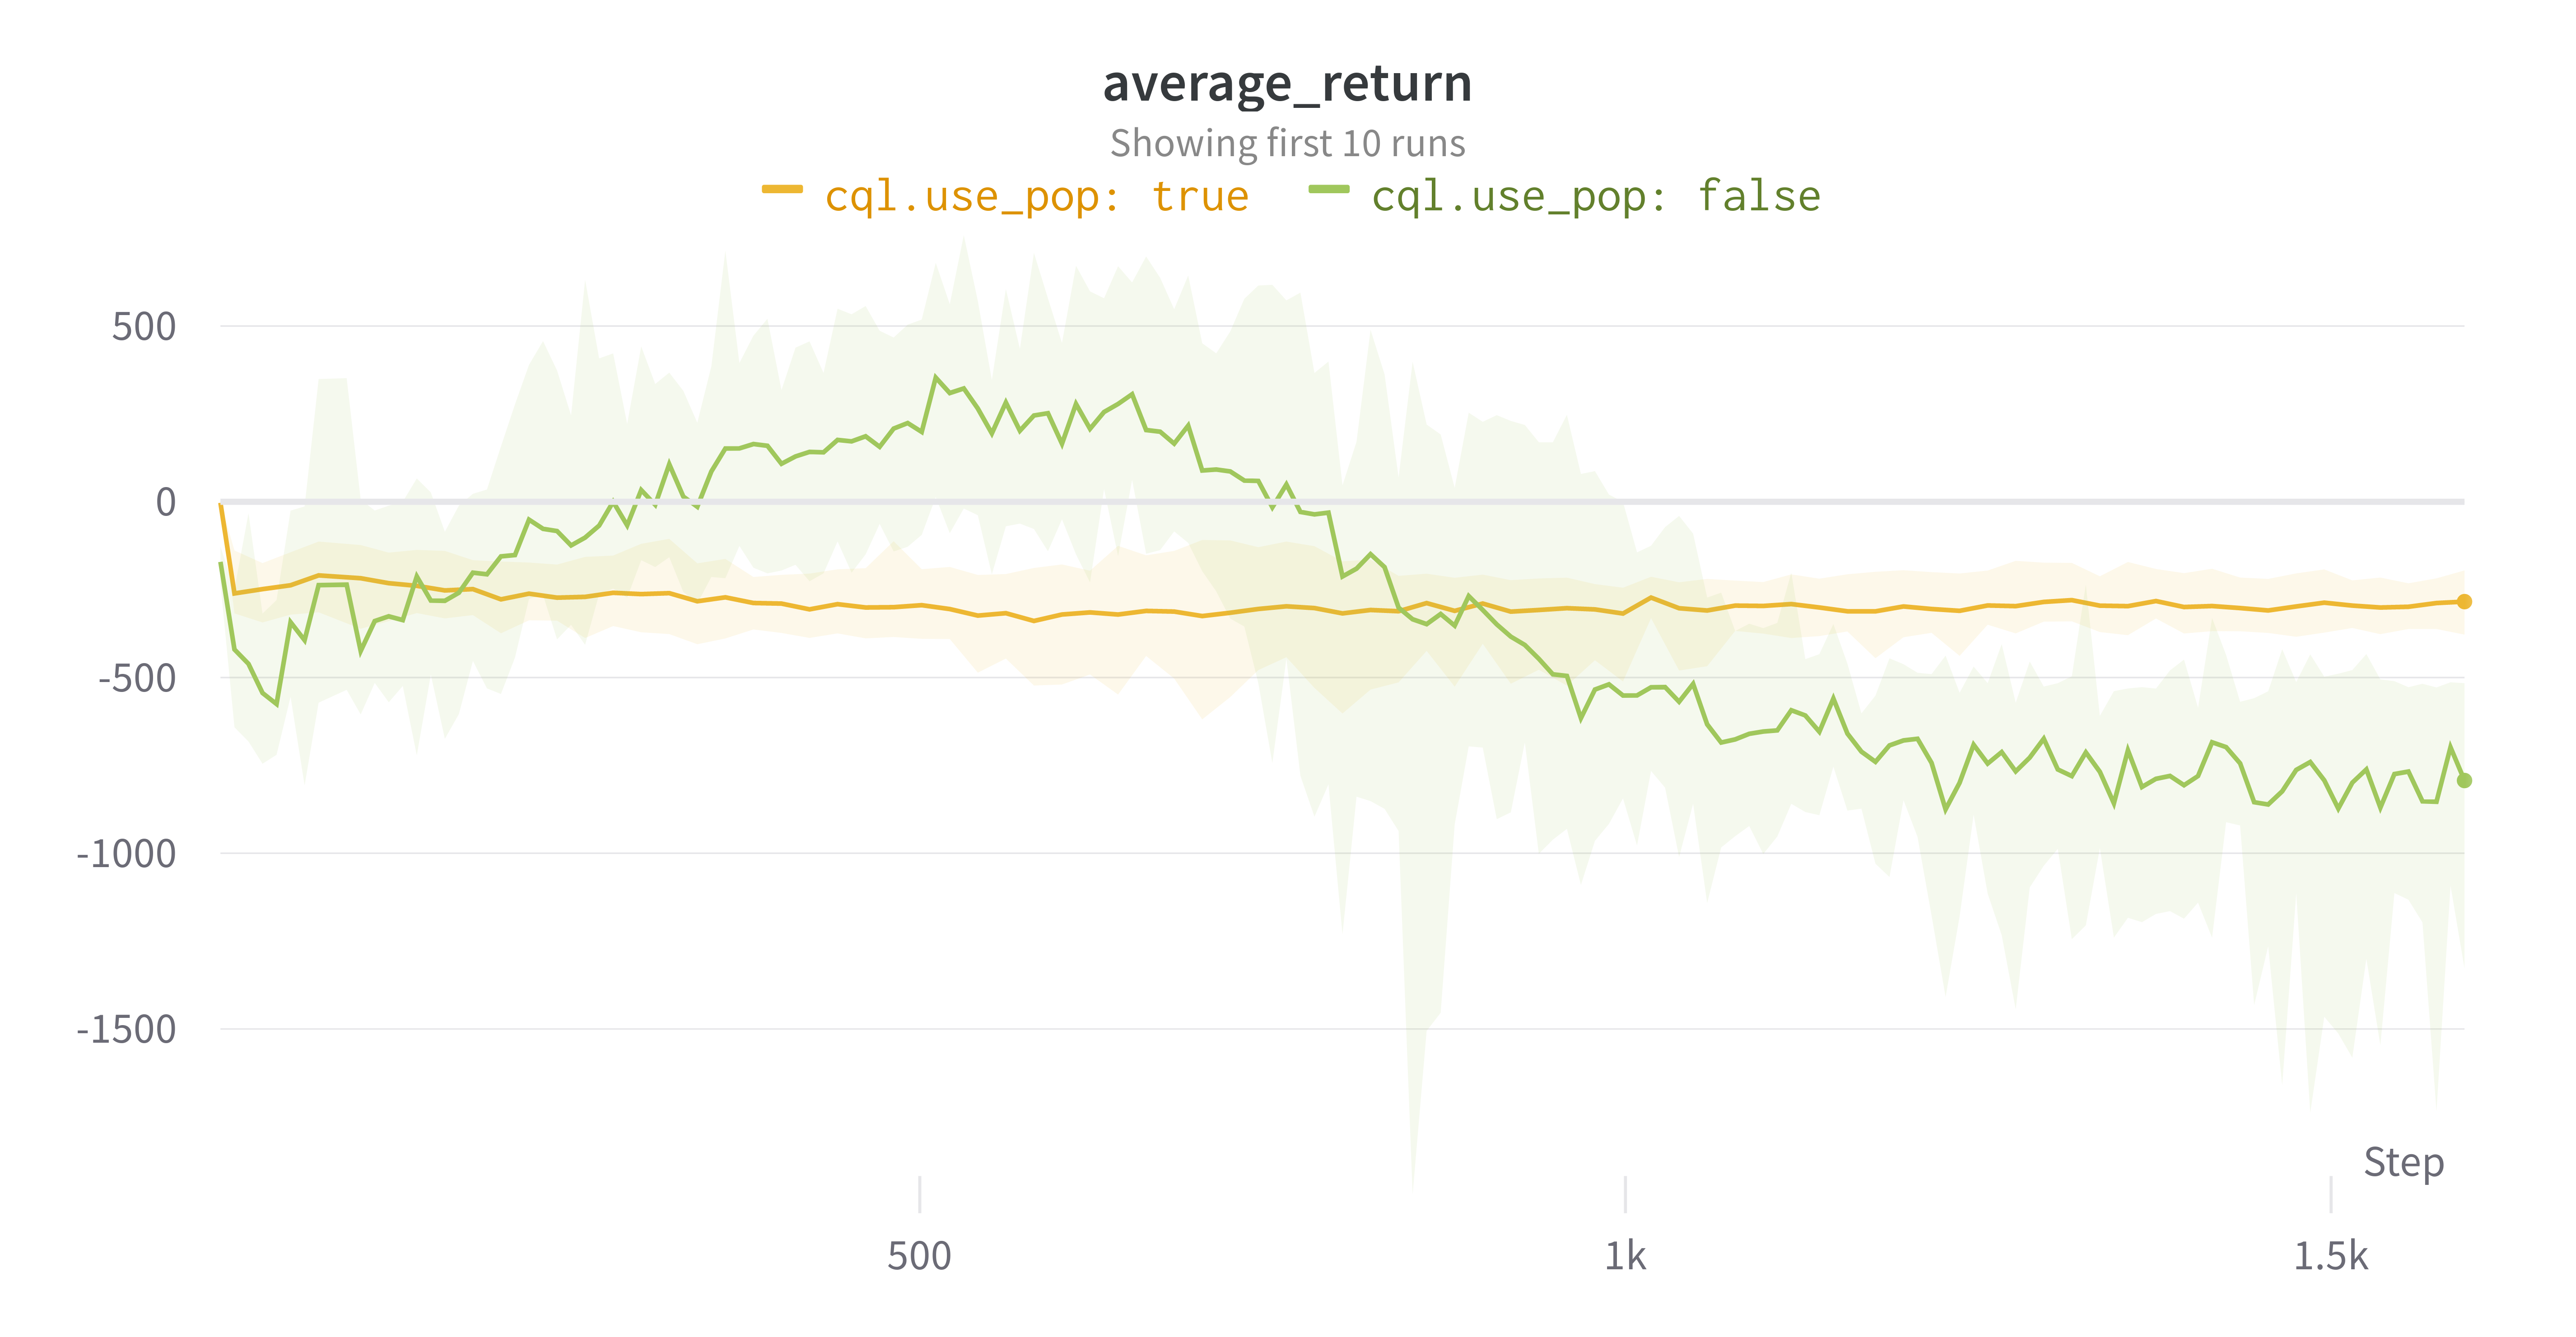
\includegraphics[width=\textwidth]{poptd/fwdback/mixedexpert.png}
  \caption{
    On custom mixed-policy dataset, POP-CQL learning has more consistent performance than naive Q learning, and is better at the limit of training. However, the highest performance achieved is by regular CQL, not POP-CQL. POP-Q can help us deal with datasets generated by vastly different policies, but more work needs to be done.
  }
  \label{fig:fwdback}
\end{figure}

\end{comment}


\section{Conclusion}
In this chapter we introduced POP-TD, a method for effective TD learning under off-policy distributions, with applications to offline RL and learning under large distribution shifts. Unlike existing emphatic TD and importance sampling methods which resample to the on-policy distribution, POP-TD resamples to the closest distribution under which TD will provably not diverge.

We present POP-TD on an existing ``deadly triad'' example in the literature, showing how the resampling process operates in theory. We extend this to a more general GridWorld-style Q-learning task which diverges under vanilla TD, but is consistently solved by POP-Q-learning.

A key strength of POP-Q-learning is that is achieves all this with a per-loop compute and memory overhead of the same order as Q-learning methods, and can be implemented and optimized in the same loop as any TD or Q-learning method. In this sense, it offers a cheap mechanism to stabilize off-policy TD, particularly in the context of offline RL.

A possible future expansion of this project is to integrate this with an existing offline RL method such as Conservative Q-Learning (CQL) and examine whether this improves performance. We propose CQL specifically because it constrains actions to remain within the support of the data, but does not explicitly constrain the distribution of states to minimize distribution shift. POP methods require adequate support (which CQL provides), and in turn are able to minimize distribution shift. This suggests that the two algorithms may have some symbiotic relationship.
